\documentclass[12pt,twoside]{mitthesis-exec}

%%%%%%%%%%%%%%%%%%%%%%%%%%%%%%%%%%%%%%%%%%%%%%%%%%%%%%%%%%%%%%%%%%%%%%%%%%%%%%%%
% PREAMBLE

\usepackage[bitstream-charter]{mathdesign} % Use BT Charter font
\usepackage[T1]{fontenc}                   % Use T1 encoding instead of OT1
\usepackage[utf8]{inputenc}                % Use UTF8 input encoding
\usepackage{microtype}                     % Improve typography
\usepackage{amsmath}                       % AMS Math extensions
\usepackage{booktabs}                      % Improve table spacing
\usepackage{graphicx}                      % Extended graphics capabilities
\usepackage{tocbibind}                     % Include listings in TOC
\usepackage[printonlyused]{acronym} % withpage: for showing page of use
\usepackage{listings}                      % Source code listings
\usepackage{caption}
\usepackage{subcaption}
\usepackage[rgb,table]{xcolor}
\usepackage{url}
\usepackage{soul}
\usepackage{array}
\usepackage{pdfpages}
\usepackage{mathtools}
\usepackage{setspace}
\usepackage{pbox}
\usepackage{tikz}
\usetikzlibrary{calc,shapes,decorations.pathreplacing,positioning}
\usepackage{pgfplots}
\usepackage{siunitx}
\usepackage{multirow}
\usepackage{breqn}

% Specialties for tables
\usepackage{array}
\newcolumntype{L}[1]{>{\raggedright\let\newline\\\arraybackslash\hspace{0pt}}m{#1}}
\newcolumntype{C}[1]{>{\centering\let\newline\\\arraybackslash\hspace{0pt}}m{#1}}
\newcolumntype{R}[1]{>{\raggedleft\let\newline\\\arraybackslash\hspace{0pt}}m{#1}}

\usepackage[breaklinks=true]{hyperref}
\hypersetup{colorlinks=true, linkcolor=black, citecolor=black, urlcolor=black,
  pdftitle={Reactor Agnostic Multi-Group Cross Section Generation for Fine-Mesh Deterministic Neutron Transport Simulations},
  pdfauthor={William Robert Dawson Boyd}
}
\pagestyle{plain}

%\usepackage{floatrow}
%\floatsetup[table]{style=plaintop}
%\floatsetup[widefigure]{margins=hangleft}

% Highlights and emphasis boxes from Bryans thesis
\usepackage[framemethod=tikz]{mdframed}
\definecolor{mitred}{rgb}{0.698,0.0314,0.216}
\definecolor{mitgray}{rgb}{0.690,0.694,0.710}
\definecolor{canyellow}{rgb}{0.933, 0.965, 0.424}
\newmdenv[nobreak=false, skipabove=2ex, skipbelow=2ex, innerlinewidth=3pt, innerlinecolor=black, backgroundcolor=mitgray!75, roundcorner=10pt, frametitlerule=true, frametitlerulewidth=2.5pt, frametitlefont=\color{white}\Large\bfseries, frametitlealignment=\centering, frametitlebackgroundcolor=mitred, frametitleaboveskip=2ex, frametitlebelowskip=2ex, innertopmargin=3ex, innerbottommargin=2ex]{highlightsbox}
\newmdenv[nobreak=false, skipabove=2ex, skipbelow=2ex, innerlinewidth=2pt, innerlinecolor=black, backgroundcolor=white, roundcorner=10pt]{emphbox}

% Appendix
\usepackage[toc,page]{appendix}

% Don't reset footnote counter between chapters
\usepackage{chngcntr}
\counterwithout{footnote}{chapter}

% Algorithm constructs
\usepackage[chapter]{algorithm} % Provides algorithm environment
\usepackage{algorithmicx}       % Provides algorithmic block
\usepackage{algpseudocode}      % Option of algorithmicx package
\renewcommand{\thealgorithm}{\thechapter-\arabic{algorithm}}
\newcommand\Algphase[1]{%
\vspace*{-.7\baselineskip}\Statex\hspace*{\dimexpr-\algorithmicindent-2pt\relax}\rule{\columnwidth}{0.4pt}%
\Statex\hspace*{-\algorithmicindent}{#1}%
\vspace*{-.7\baselineskip}\Statex\hspace*{\dimexpr-\algorithmicindent-2pt\relax}\rule{\columnwidth}{0.4pt}%
}
\newcommand{\algrule}[1][.4pt]{\par\vskip.5\baselineskip\hrule height #1\par\vskip.5\baselineskip}

% Configure captions
\captionsetup{labelfont=bf, labelsep=colon}
\captionsetup[algorithm]{labelfont=bf, labelsep=colon}

% Use Latin Modern for typewriter fonts
\renewcommand{\ttdefault}{lmtt}

% Add \unit macro
\newcommand{\unit}[1]{\ensuremath{\, \mathrm{#1}}}

\definecolor{gray}{rgb}{0.4,0.4,0.4}
\definecolor{darkblue}{rgb}{0.0,0.0,0.6}
\definecolor{cyan}{rgb}{0.0,0.6,0.6}
\lstset{
  basicstyle=\footnotesize\ttfamily,
  columns=fullflexible,
  showstringspaces=false,
  commentstyle=\color{gray}\upshape,
  frame=single,
  xleftmargin=0.55in
}

\lstdefinelanguage{XML}
{
  morestring=[b]",
  morestring=[s]{>}{<},
  morecomment=[s]{<?}{?>},
  morecomment=[s]{<!--}{-->},
  stringstyle=\color{black},
  identifierstyle=\color{darkblue},
  keywordstyle=\color{cyan},
  morekeywords={}
}

\setcounter{secnumdepth}{4}
\setcounter{tocdepth}{3}

\renewcommand{\contentsname}{Table of Contents}
\renewcommand{\bibname}{References}

\makeatletter \renewcommand\thealgorithm{\arabic{algorithm}} \@addtoreset{algorithm}{chapter} \makeatother

\begin{document}

%%%%%%%%%%%%%%%%%%%%%%%%%%%%%%%%%%%%%%%%%%%%%%%%%%%%%%%%%%%%%%%%%%%%%%%%%%%%%%%%
% TITLE PAGE

% -*-latex-*-
% 
% For questions, comments, concerns or complaints:
% thesis@mit.edu
% 
%
% $Log: cover.tex,v $
% Revision 1.8  2008/05/13 15:02:15  jdreed
% Degree month is June, not May.  Added note about prevdegrees.
% Arthur Smith's title updated
%
% Revision 1.7  2001/02/08 18:53:16  boojum
% changed some \newpages to \cleardoublepages
%
% Revision 1.6  1999/10/21 14:49:31  boojum
% changed comment referring to documentstyle
%
% Revision 1.5  1999/10/21 14:39:04  boojum
% *** empty log message ***
%
% Revision 1.4  1997/04/18  17:54:10  othomas
% added page numbers on abstract and cover, and made 1 abstract
% page the default rather than 2.  (anne hunter tells me this
% is the new institute standard.)
%
% Revision 1.4  1997/04/18  17:54:10  othomas
% added page numbers on abstract and cover, and made 1 abstract
% page the default rather than 2.  (anne hunter tells me this
% is the new institute standard.)
%
% Revision 1.3  93/05/17  17:06:29  starflt
% Added acknowledgements section (suggested by tompalka)
% 
% Revision 1.2  92/04/22  13:13:13  epeisach
% Fixes for 1991 course 6 requirements
% Phrase "and to grant others the right to do so" has been added to 
% permission clause
% Second copy of abstract is not counted as separate pages so numbering works
% out
% 
% Revision 1.1  92/04/22  13:08:20  epeisach

% NOTE:
% These templates make an effort to conform to the MIT Thesis specifications,
% however the specifications can change.  We recommend that you verify the
% layout of your title page with your thesis advisor and/or the MIT 
% Libraries before printing your final copy.
\title{Reactor Agnostic Multi-Group Cross Section Generation for Fine Mesh Deterministic Neutron Transport Simulations}

\author{William Robert Dawson Boyd III}

% If you wish to list your previous degrees on the cover page, use the 
% previous degrees command:
\prevdegrees{B.S., Georgia Institute of Technology (2010) \\
             M.S., Massachusetts Institute of Technology (2014)}

% You can use the \\ command to list multiple previous degrees
%       \prevdegrees{B.S., University of California (1978) \\
%                    S.M., Massachusetts Institute of Technology (1981)}
\department{Department of Nuclear Science and Engineering}

% If the thesis is for two degrees simultaneously, list them both
% separated by \and like this:
% \degree{Doctor of Philosophy \and Master of Science}
\degree{Doctor of Philosophy in Nuclear Science and Engineering}

% As of the 2007-08 academic year, valid degree months are September, 
% February, or June.  The default is June.
\degreemonth{February}
\degreeyear{2016}
\thesisdate{November 4, 2016}

%% By default, the thesis will be copyrighted to MIT.  If you need to copyright
%% the thesis to yourself, just specify the `vi' documentclass option.  If for
%% some reason you want to exactly specify the copyright notice text, you can
%% use the \copyrightnoticetext command.  
%\copyrightnoticetext{\copyright IBM, 1990.  Do not open till Xmas.}

% If there is more than one supervisor, use the \supervisor command
% once for each.
\supervisor{Kord Smith}{KEPCO Professor of the Practice of Nuclear Science and Engineering} 
% Deparment of Nuclear Science and Engineering
\supervisor{Benoit Forget}{Associate Professor of Nuclear Science and Engineering} 
% Department of Nuclear Science & Engineering

% This is the department committee chairman, not the thesis committee
% chairman.  You should replace this with your Department's Committee
% Chairman.
%\chairman{Ju Li}{Professor of Nuclear Science and Engineering}{Chair, Committee on Graduate Students}

% Make the titlepage based on the above information.  If you need
% something special and can't use the standard form, you can specify
% the exact text of the titlepage yourself.  Put it in a titlepage
% environment and leave blank lines where you want vertical space.
% The spaces will be adjusted to fill the entire page.  The dotted
% lines for the signatures are made with the \signature command.
\maketitle

% The abstractpage environment sets up everything on the page except
% the text itself.  The title and other header material are put at the
% top of the page, and the supervisors are listed at the bottom.  A
% new page is begun both before and after.  Of course, an abstract may
% be more than one page itself.  If you need more control over the
% format of the page, you can use the abstract environment, which puts
% the word "Abstract" at the beginning and single spaces its text.

%% You can either \input (*not* \include) your abstract file, or you can put
%% the text of the abstract directly between the \begin{abstractpage} and
%% \end{abstractpage} commands.



% First copy: start a new page, and save the page number.
%\cleardoublepage

% Uncomment the next line if you do NOT want a page number on your
% abstract and acknowledgments pages.
%\setcounter{savepage}{\thepage}
%\begin{abstractpage}
%\begin{abstractpage}

The development of high fidelity multi-group neutron transport-based simulation tools for full core Light Water Reactor (LWR) analysis has been a long-standing goal of the reactor physics community. While direct transport simulations have previously been far too computationally expensive, advances in computer hardware have allowed large scale simulations to become feasible. Therefore, many have focused on developing full core neutron transport solvers that do not incorporate the approximations and assumptions of traditional nodal diffusion solvers. 

Due to the computational expense of direct full core 3D deterministic neutron transport methods, many have focused on 2D/1D methods which solve 3D problems as a coupled system of radial and axial transport problems. However, the coupling of radial and axial problems also introduces approximations. Instead, the work in this thesis focuses on explicitly solving the 3D deterministic neutron transport equations with the Method of Characteristics (MOC).

MOC has been widely used for 2D lattice physics calculations due to its ability to accurately and efficiently simulate reactor physics problems with explicit geometric detail. The work in this thesis strives to overcome the significant computational cost of solving the 3D MOC equations by implementing efficient track generation, axially extruded ray tracing, Coarse Mesh Finite Difference (CMFD) acceleration, linear track-based source approximations, and scalable domain decomposition. 

Additionally, significant attention has been be given to complications that arise in full core simulations with transport-corrected cross-sections. The convergence behavior of transport methods is analyzed, leading to a new strategy for stabilizing the source iteration scheme for neutron transport simulations. The methods are incorporated into the OpenMOC reactor physics code and simulation results are presented for the full core BEAVRS LWR benchmark. Parameter refinement studies and comparisons with reference OpenMC Monte Carlo solutions show that converged full core 3D MOC simulations are feasible on modern supercomputers for the first time.

%However, 3D full core LWR simulations present significant challenges due to greatly increased computational cost.

%The Method of Characteristics (MOC) has seen wide interest in reactor physics because of its accuracy and efficiency in computing lattice physics problems. While most of its use has been in solving 2D problems, there has been recent interest in extending MOC to 3D in order to more accurately calculate 3D power distributions in LWRs. While the method is naturally extensible to 3D, it presents significant computational difficulties. Methods will be presented which mitigate the computational difficulties of 3D MOC by using domain decomposition, efficient track generation, axially extruded ray tracing, CMFD acceleration, and a linear source approximation. Significant attention will be given to complications that arise in full core simulations. 3D MOC results will be presented for the full core simulation of the BEAVRS benchmark, showing that 3D MOC can be a viable tool for anal

\end{abstractpage}
%\end{abstractpage}




% Additional copy: start a new page, and reset the page number.  This way,
% the second copy of the abstract is not counted as separate pages.
% Uncomment the next 6 lines if you need two copies of the abstract
% page.
% \setcounter{page}{\thesavepage}
% \begin{abstractpage}
% \begin{abstractpage}

The development of high fidelity multi-group neutron transport-based simulation tools for full core Light Water Reactor (LWR) analysis has been a long-standing goal of the reactor physics community. While direct transport simulations have previously been far too computationally expensive, advances in computer hardware have allowed large scale simulations to become feasible. Therefore, many have focused on developing full core neutron transport solvers that do not incorporate the approximations and assumptions of traditional nodal diffusion solvers. 

Due to the computational expense of direct full core 3D deterministic neutron transport methods, many have focused on 2D/1D methods which solve 3D problems as a coupled system of radial and axial transport problems. However, the coupling of radial and axial problems also introduces approximations. Instead, the work in this thesis focuses on explicitly solving the 3D deterministic neutron transport equations with the Method of Characteristics (MOC).

MOC has been widely used for 2D lattice physics calculations due to its ability to accurately and efficiently simulate reactor physics problems with explicit geometric detail. The work in this thesis strives to overcome the significant computational cost of solving the 3D MOC equations by implementing efficient track generation, axially extruded ray tracing, Coarse Mesh Finite Difference (CMFD) acceleration, linear track-based source approximations, and scalable domain decomposition. 

Additionally, significant attention has been be given to complications that arise in full core simulations with transport-corrected cross-sections. The convergence behavior of transport methods is analyzed, leading to a new strategy for stabilizing the source iteration scheme for neutron transport simulations. The methods are incorporated into the OpenMOC reactor physics code and simulation results are presented for the full core BEAVRS LWR benchmark. Parameter refinement studies and comparisons with reference OpenMC Monte Carlo solutions show that converged full core 3D MOC simulations are feasible on modern supercomputers for the first time.

%However, 3D full core LWR simulations present significant challenges due to greatly increased computational cost.

%The Method of Characteristics (MOC) has seen wide interest in reactor physics because of its accuracy and efficiency in computing lattice physics problems. While most of its use has been in solving 2D problems, there has been recent interest in extending MOC to 3D in order to more accurately calculate 3D power distributions in LWRs. While the method is naturally extensible to 3D, it presents significant computational difficulties. Methods will be presented which mitigate the computational difficulties of 3D MOC by using domain decomposition, efficient track generation, axially extruded ray tracing, CMFD acceleration, and a linear source approximation. Significant attention will be given to complications that arise in full core simulations. 3D MOC results will be presented for the full core simulation of the BEAVRS benchmark, showing that 3D MOC can be a viable tool for anal

\end{abstractpage}
% \end{abstractpage}

\cleardoublepage

%%%%%%%%%%%%%%%%%%%%%%%%%%%%%%%%%%%%%%%%%%%%%%%%%%%%%%%%%%%%%%%%%%%%%%
% -*-latex-*-


\title{EXECUTIVE SUMMARY \\~\\ Reactor Agnostic Multi-Group Cross Section Generation for Fine-Mesh Deterministic Neutron Transport Simulations}

\author{William Robert Dawson Boyd III}
\prevdegrees{B.S., Georgia Institute of Technology (2010) \\
             M.S., Massachusetts Institute of Technology (2014)}
\department{Department of Nuclear Science and Engineering}
\degree{Doctor of Philosophy in Nuclear Science and Engineering}

\degreemonth{February}
\degreeyear{2017}
\thesisdate{November 4, 2016}

%\supervisor{Benoit Forget}{Associate Professor of Nuclear Science and Engineering}
%\reader{Kord S. Smith}{KEPCO Professor of the Practice of Nuclear Science and Engineering}
%\chairman{Emilio Bagglietto}{Associate Professor of Nuclear Science and Engineering}


%%%%%%%%%%%%%%%%%%%%%%%%%%%%%%%%%%%%%%%%%%%%%%%%%%%%%%%%%%%%%%%%%%%%%%%%%%%%%%%%
%%%%%%%%%%%%%%%%%%%%%%%%%%%%%%%%%%%%%%%%%%%%%%%%%%%%%%%%%%%%%%%%%%%%%%%%%%%%%%%%
% ABSTRACT

%\setcounter{savepage}{\thepage}

\begin{abstractpage}

The development of high fidelity multi-group neutron transport-based simulation tools for full core Light Water Reactor (LWR) analysis has been a long-standing goal of the reactor physics community. While direct transport simulations have previously been far too computationally expensive, advances in computer hardware have allowed large scale simulations to become feasible. Therefore, many have focused on developing full core neutron transport solvers that do not incorporate the approximations and assumptions of traditional nodal diffusion solvers. 

Due to the computational expense of direct full core 3D deterministic neutron transport methods, many have focused on 2D/1D methods which solve 3D problems as a coupled system of radial and axial transport problems. However, the coupling of radial and axial problems also introduces approximations. Instead, the work in this thesis focuses on explicitly solving the 3D deterministic neutron transport equations with the Method of Characteristics (MOC).

MOC has been widely used for 2D lattice physics calculations due to its ability to accurately and efficiently simulate reactor physics problems with explicit geometric detail. The work in this thesis strives to overcome the significant computational cost of solving the 3D MOC equations by implementing efficient track generation, axially extruded ray tracing, Coarse Mesh Finite Difference (CMFD) acceleration, linear track-based source approximations, and scalable domain decomposition. 

Additionally, significant attention has been given to complications that arise in full core simulations with transport-corrected cross-sections. The convergence behavior of transport methods is analyzed, leading to a new strategy for stabilizing the source iteration scheme for neutron transport simulations. The methods are incorporated into the OpenMOC reactor physics code and simulation results are presented for the full core BEAVRS LWR benchmark. Parameter refinement studies and comparisons with reference OpenMC Monte Carlo solutions show that converged full core 3D MOC simulations are feasible on modern supercomputers for the first time.

%However, 3D full core LWR simulations present significant challenges due to greatly increased computational cost.


%The Method of Characteristics (MOC) has seen wide interest in reactor physics because of its accuracy and efficiency in computing lattice physics problems. While most of its use has been in solving 2D problems, there has been recent interest in extending MOC to 3D in order to more accurately calculate 3D power distributions in LWRs. While the method is naturally extensible to 3D, it presents significant computational difficulties. Methods will be presented which mitigate the computational difficulties of 3D MOC by using domain decomposition, efficient track generation, axially extruded ray tracing, CMFD acceleration, and a linear source approximation. Significant attention will be given to complications that arise in full core simulations. 3D MOC results will be presented for the full core simulation of the BEAVRS benchmark, showing that 3D MOC can be a viable tool for analysis of PWR reactors.

\end{abstractpage}


\singlespacing 

%%%%%%%%%%%%%%%%%%%%%%%%%%%%%%%%%%%%%%%%%%%%%%%%%%%%%%%%%%%%%%%%%%%%%%%%%%%%%%%%
\section*{Introduction}

%%%%%%%%%%%%%%%%%%%%%%%%%%%%%%%%%%%%%%%
\subsection*{Background and Motivation}

The development and deployment of nuclear reactor core physics simulations is governed by tradeoffs between accuracy and speed. High-fidelity simulations are accurate and flexible but require significant computational resources, while the approximations made by low-fidelity methods reduce the number of variables which greatly improves the time-to-solution. As a result, it is common to employ a mix of high- and low-fidelity tools for reactor analysis -- for example, high-fidelity tools are frequently used to inform and benchmark low-fidelity models for use within a narrow envelope of design parameters. This thesis develops a new approach within the same vein by employing continuous energy Monte Carlo (MC) neutron transport simulations to generate accurate multi-group cross sections (MGXS) for computationally efficient whole-core deterministic transport methods. These methods replace engineering judgment with machine learning which processes ``noisy'' tally data computed by an unconverged whole-core MC simulation.

%Unlike the today's multi-level approaches for MGXS generation, the methods developed in this work remove the need for engineering judgment and instead infer MGXS from ``noisy'' MC tally data computed by a single unconverged whole-core MC simulation.

%\textbf{This thesis is motivated by the desire to obtain Monte Carlo-quality solutions with computationally efficient deterministic neutron transport methods.}

This thesis investigates the use of Monte Carlo methods to generate MGXS, such as the U-235 fission MGXS illustrated in Fig.~\ref{fig:u235-sigf}, for reactor core analysis. Monte Carlo presents a natural approach to replace engineering prescriptions to approximate the flux with a stochastic realization of the exact flux. The advantage of a MC-based approach is that all of the relevant physics modeled in MC may be directly embedded into MGXS. This improvement in accuracy comes at the computational expense of converging group constant tallies to acceptably low uncertainties. MC methods have increasingly been used to generate few group constants for coarse mesh diffusion, most notably by the Serpent MC code~\cite{serpent2013manual}. However, there exist few rigorous and comprehensive analyses of MGXS generation for heterogeneous fine-mesh deterministic transport methods~\cite{redmond1997multigroup,cai2014condensation,nelson2014improved}. \textbf{This thesis develops and evaluates MC-based methods to generate MGXS for fine-mesh deterministic neutron transport codes.}

\begin{figure}[h!]
\centering
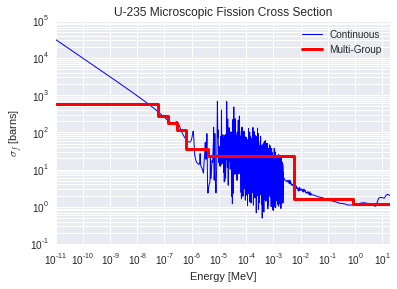
\includegraphics[width=0.65\linewidth]{figures/intro/u235-ce-mg-xs}
\caption[U-235 continuous energy and multi-group fission cross section]{U-235 continuous energy and 16-group fission cross section.}
\label{fig:u235-sigf}
\end{figure}

In addition, MC-based MGXS generation methods to date have retained the multi-level geometric framework illustrated in Fig.~\ref{fig:multi-level-flow-chart} to tabulate MGXS for individual reactor components -- such as infinite fuel pins and/or assemblies -- for subsequent use in whole-core multi-group calculations. The multi-level approach is inspired by legacy MGXS generation techniques which apply high-fidelity models of the energy self-shielding physics to low-fidelity geometric models of unique core components. The complexity of the energy treatment is then reduced at each level as larger and more complex geometric models are considered. \textbf{This thesis replaces the multi-level framework in place of a whole-core MC calculation which simultaneously accounts for all energy and spatial effects with a single simulation of the complete heterogeneous geometry.}

\begin{figure}[h!]
\centering
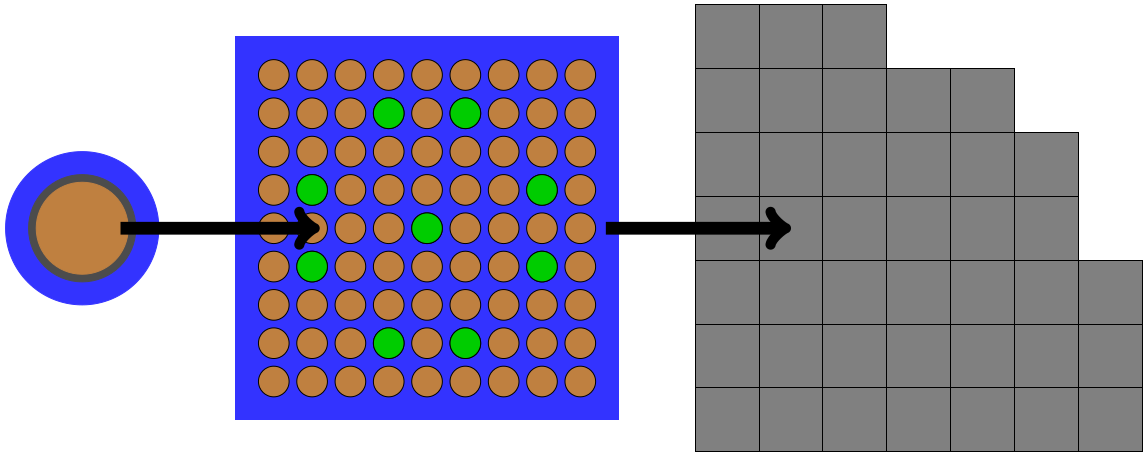
\includegraphics[width=0.9\linewidth]{figures/intro/multi-step-flow-chart}
\caption[Multi-level approach to reactor analysis]{Current multi-level framework for reactor analysis.}
\label{fig:multi-level-flow-chart}
\end{figure}

In theory, whole-core MC calculations can be used to tally MGXS in each spatial zone (\textit{e.g.}, 100 axial depletion zones within each of 50,000+ fuel pins in a PWR core) to account for the spatial variation of the flux. However, such simulations have not been employed for practical reasons -- in particular, the computational expense of performing such calculations has been prohibitive for MC codes until recent years. Furthermore, roughly the same number of particle histories would be required to converge the MGXS tallies in each spatial zone as would be required for a direct whole-core calculation by MC. \textbf{Therefore, a new method is required to accelerate the convergence of the MGXS tallies in each fine-mesh region in order for MC to be practical for reactor agnostic fine-mesh MGXS generation.}

This thesis proposes both engineering-based clustering and statistical clustering methods to accelerate the convergence of whole-core MC calculations for MGXS generation. This novel approach relies on the fact that many distinct spatial zones across a reactor core experience similar if not identical spatial and energy self-shielding effects, and therefore have similar if not identical MGXS. The stochastic nature of MC simulations will contribute statistical ``noise'' to the tally estimates for the MGXS. As a result, the MGXS estimates for similarly self-shielded spatial zones form clusters which converge as more particle histories are simulated. \textbf{The goal of this thesis is to develop and apply machine learning algorithms to identify MGXS clusters from ``noisy'' Monte Carlo tally data. This methodology aims to generate MGXS for deterministic neutron transport codes in a reactor agnostic and computationally efficient manner.}

%%%%%%%%%%%%%%%%%%%%%%%%
\subsection*{Objectives}

The subject matter of this thesis is organized along two main themes:

\begin{itemize}
\item \textbf{\textit{Approximation Error}} -- Quantify and diagnose approximation error in MGXS generated from MC methods for simple heterogeneous benchmark problems.
\item \textbf{\textit{Statistical Clustering}} -- Develop statistical clustering methods to accelerate the convergence of MGXS on heterogeneous MC tally meshes.
\end{itemize}

The first theme of this thesis rigorously assesses the efficacy of MGXS generation with MC for fine-mesh transport calculations. Some of the approximations made by MC-based MGXS generation are quantified, including an in-depth analysis of systematic bias resulting from constant-in-angle total MGXS. The second theme develops a new methodology called \textit{inferential multi-group cross sections} (\textit{i}MGXS) to simultaneously capture local and global spatial self-shielding effects in MGXS for whole-core calculations. The \textit{i}MGXS scheme applies statistical clustering methods to accelerate the convergence of MGXS tallied on fine, heterogeneous spatial meshes in Monte Carlo. The \textit{i}MGXS scheme is evaluated for six heterogeneous PWR benchmarks to quantify its accuracy and convergence relative to alternative schemes for MC-based MGXS generation.

%%%%%%%%%%%%%%%%%%%%%%%%%%%%%%%%%%%%%%%%%%%%%%%%%%%%%%%%%%%%%%%%%%%%%%%%%%%%%%%%
\section*{Software Infrastructure: A Simulation Triad}

This thesis investigates Monte Carlo as a means to generate multi-group cross sections for fine-mesh transport codes. This work required the development of a ``simulation triad'' encompassing three primary codes as illustrated in Fig.~\ref{fig:simulation-triad}. First, the OpenMC Monte Carlo code~\cite{romano2013openmc} was utilized to generate multi-group cross sections. Second, the MGXS were used by the OpenMOC code~\cite{boyd2014openmoc} for deterministic multi-group transport calculations. Finally, the OpenCG library~\cite{boyd2015opencg} enabled the processing and transfer of tally data on combinatorial geometry (CG) meshes between OpenMC and OpenMOC. The following sections summarize the author's contributions to each component code in the simulation triad to support the objectives of this thesis.

\begin{figure}[h!]
  \centering
  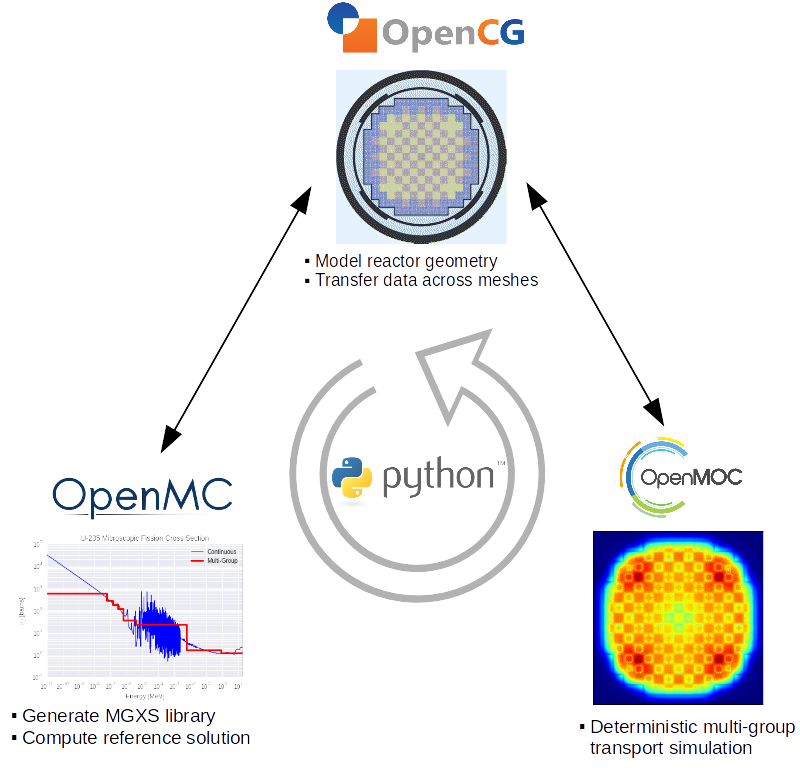
\includegraphics[width=0.95\linewidth]{figures/workflow/triad/simulation-triad}
\caption[A simulation triad of OpenMC, OpenMOC and OpenCG]{A simulation triad consisting of the OpenMC, OpenMOC and OpenCG codes ``glued'' together with Python formed the foundation for this thesis research.}
\label{fig:simulation-triad}
\end{figure}

%%%%%%%%%%%%%%%%%%%%
\subsection*{OpenMC}

The OpenMC code is a continuous energy Monte Carlo neutron transport code~\cite{romano2013openmc} with support for general constructive solid geometry models. This thesis designed and implemented a fully-featured OpenMC Python API to enable the processing of large tally datasets to generate MGXS. In addition, a distributed cell tally algorithm~\cite{lax2014distribcell} was implemented in OpenMC to compute MGXS across repeated fuel pin cells in reactor core geometries. Finally, an option for isotropic in lab scattering was implemented and used to generate MGXS. The isotropic scattering feature enabled ``apples-to-apples'' comparisons between the reference eigenvalues and reaction rates produced by OpenMC and those computed from isotropic multi-group calculations with OpenMOC. 

%In total, the author contributed over 20,000 lines of Python and 2,000 lines of Fortran code to the open source release version of OpenMC to support this work.

%%%%%%%%%%%%%%%%%%%%%
\subsection*{OpenMOC}

The OpenMOC code is a multi-group neutron transport code implementing the deterministic Method of Characteristics (MOC)~\cite{boyd2014openmoc}. The OpenMOC code is capable of performing 2D MOC transport calculations for LWR core configurations. The \texttt{openmoc.materialize} Python module was implemented to automate the loading MGXS data into OpenMOC \texttt{Material} objects. The module is designed to support the large MGXS libraries generated by OpenMC. In addition, a new module was implemented  to interface with the OpenCG region differentiation algorithm, which constructed ``clustered geometries'' for OpenMOC. Finally, a scheme to compute SuPerHomog\'{e}n\'{e}isation (SPH) factors to ensure reaction rate consistency with OpenMC was implemented in OpenMOC. 

%In total, the author contributed over 15,000 lines of C++ and nearly 20,000 lines of Python code to the open source release version of OpenMOC to support this work.

%%%%%%%%%%%%%%%%%%%%
\subsection*{OpenCG}

A new combinatorial geometry (CG) Python library called OpenCG~\cite{boyd2015opencg} was developed to construct complicated reactor geometries for OpenMOC. Two novel algorithms known as Local Neighbor Symmetry (LNS) and region differentiation were developed in OpenCG to support this thesis. The LNS algorithm analyzes a combinatorial geometry to identify neighbor cells, or pairs of cells which are adjacent to one another. The LNS algorithm is analogous to the geometric templates used in lattice physics codes such as CASMO~\cite{edenius1995casmo} to identify fuel pins which have similar resonance self-shielding Dancoff factors. The region differentiation algorithm was developed to efficiently construct geometries which represent the assignment of MGXS to arbitrary ``clusters'' of fuel pins. The differentiated geometries are exported to OpenMOC for deterministic neutron transport calculations. 

%The author contributed over 10,000 lines of Python code in OpenCG to support this work.


%%%%%%%%%%%%%%%%%%%%%%%%%%%%%%%%%%%%%%%%%%%%%%%%%%%%%%%%%%%%%%%%%%%%%%%%%%%%%%%%%
%\section*{Angular-Dependent MGXS and SPH Factors}
%
%%%%%%%%%%%%%%%%%%%%%%%%%%%%%%%%%%%%%%%%%%%%%%
%\subsection*{Flux Separability Approximation}
%
%\begin{dmath}
%\label{eqn:sigt-flux-separable}
%\Sigma_{t,g}(\mathbf{r}) = \frac{\int\displaylimits_{E_{g}}^{E_{g-1}} \Sigma_{t}(\mathbf{r},E)\psi(\mathbf{r},\mathbf{\Omega},\mathrm{d}E)}{\psi_{g}(\mathbf{r},\mathbf{\Omega})} \approx \frac{\int\displaylimits_{E_{g}}^{E_{g-1}} \Sigma_{t}(\mathbf{r},E)\phi(\mathbf{r},E)}{\phi_{g}(\mathbf{r})}
%\end{dmath}
%
%\clearpage
%
%%%%%%%%%%%%%%%%%%%%%%%%%%%%%%%%%%%%%%%%%%%
%\subsection*{Energy-Dependent Flux Errors}
%
%\begin{figure}[h!]
%\centering
%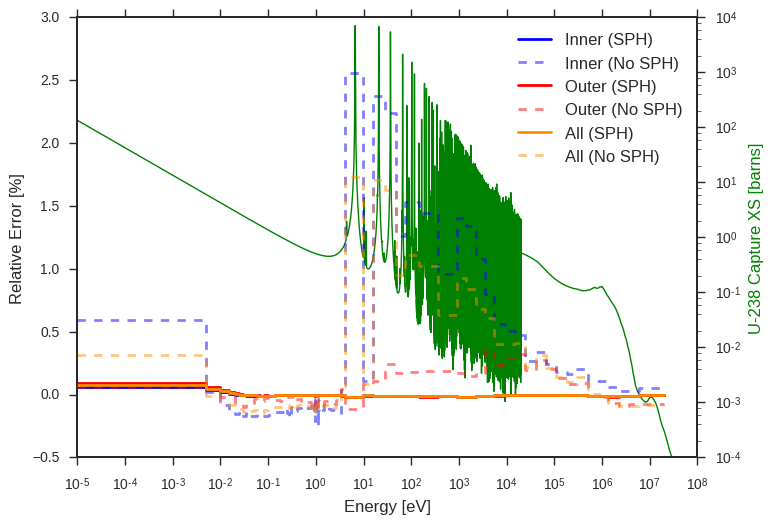
\includegraphics[width=\linewidth]{figures/sph/pin-cell/rel-err-inner-outer}
%\caption[Flux relative error by energy group with SPH]{The energy-dependent relative error of the 70-group OpenMOC scalar flux with respect to the OpenMC flux in a fuel pin for the innermost, outermost and all FSRs.}
%\label{fig:rel-err-energy}
%\end{figure}
%
%\clearpage

%%%%%%%%%%%%%%%%%%%%%%%%%%%%%%%%%%%%%
%\subsection*{Angular-Dependent MGXS}
%
%\begin{figure}[h]
%\begin{subfigure}{.5\textwidth}
%  \centering
%  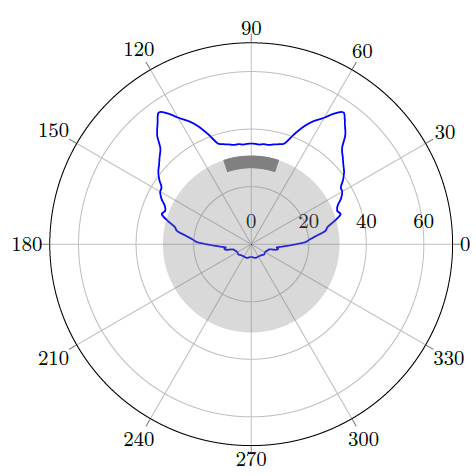
\includegraphics[width=\linewidth]{figures/sph/batman-1}
%  \caption{}
%  \label{fig:batman-plots-a}
%\end{subfigure}
%\begin{subfigure}{.5\textwidth}
%  \centering
%  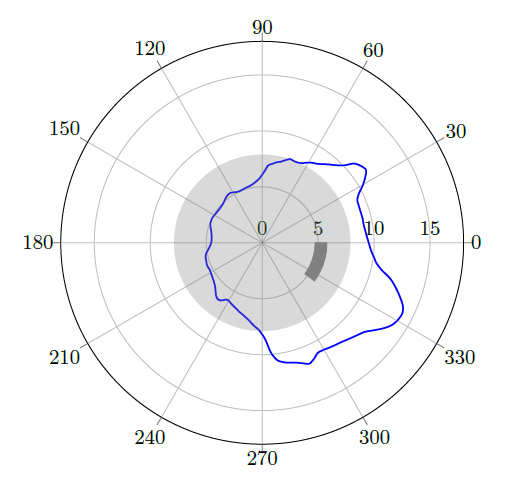
\includegraphics[width=\linewidth]{figures/sph/batman-2}
%  \caption{}
%  \label{fig:batman-plots-b}
%\end{subfigure}
%\caption[Angular-dependent capture MGXS]{Angular-dependent capture MGXS for the 6.67 eV resonance group as a function of azimuthal angle for two different FSRs. The radial axis is given in units of barns and the azimuthal axis in units of degrees. \textit{Image courtesy of N. Gibson~\cite{gibson2016thesis}.}}
%\label{fig:batman-plots}
%\end{figure}
%
%\clearpage
%
%%%%%%%%%%%%%%%%%%%%%%%%%%%%%%%%%%%%%%%%%%%%%%%%%%%
%\subsection*{SuPerHomog\'{e}n\'{e}isation Factors}
%
%-SPH factors were first proposed by H\'{e}bert~\cite{hebert1993consistent} to preserve reaction rates during energy condensation and spatial homogenization \\
%-SPH factor algorithm requires knowledge of a reference source that is used in a multi-group fixed source solver to derive multiplicative factors that adjust the total MGXS to force neutron balance \\
%
%\begin{dmath}
%\label{eqn:sph-transport-eqn-iterate}
%\mathbf{\Omega} \cdot \nabla \psi_{g}^{(n)}(\mathbf{r},\mathbf{\Omega}) + \mu_{k,g}^{(n-1)}\Sigma_{t,k,g}\psi_{g}^{(n)}(\mathbf{r},\mathbf{\Omega}) = Q_{k,g}(\mathbf{\Omega})
%\end{dmath}
%
%\begin{dmath}
%\label{eqn:sph-update-sigt}
%\Sigma_{t,k,g}^{(n)} = \mu_{k,g}^{(n-1)}\Sigma_{t,k,g}^{(0)}
%\end{dmath}
%
%\begin{algorithm}[h]
%\caption{SPH Factor Algorithm}
%\label{alg:sph}
%\begin{algorithmic}[1]
%%  \State Initialize MGXS from MC tallies
%%  \State Compute neutron source from MC flux and MGXS
%  \State Initialize SPH factors to unity
%  \While{SPH factors are not converged}
%    \State Update MGXS with SPH factors \Comment{Eqn.~\ref{eqn:sph-update-sigt}}
%    \State Solve fixed source transport problem \Comment{Eqn.~\ref{eqn:sph-transport-eqn-iterate}}
%    \State Compute new SPH factors
%  \EndWhile
%  \State Compute final MGXS with SPH factors \Comment{Eqn.~\ref{eqn:sph-update-sigt}}
%\end{algorithmic}
%\end{algorithm}
%
%\begin{table}[h!]
%  \centering
%  \caption[Eigenvalues with and without SPH factors for a fuel pin]{The impact of SPH factors on the eigenvalue bias $\Delta\rho$ with varying energy group structures for a fuel pin.}  
%  \label{table:sph-keff}
%  \vspace{6pt}
%  \begin{tabular}{c S[table-format=6.1] S[table-format=6.1]}
%  \toprule
%  & \multicolumn{2}{c}{{\bf $\boldsymbol{\Delta\rho}$ [pcm]}} \\
%  \cline{2-3}
%  \multirow{-2}{*}{{\bf \# Groups}} &
%  \multicolumn{1}{c}{{\bf Without SPH}} &
%  \multicolumn{1}{c}{{\bf With SPH}} \\
%  \midrule
%1 & 66 & -14 \\
%2 & 34 & -6\\
%4 & -57 & 1 \\
%8 & -102 & 2 \\
%16 & -111 & 4 \\
%25 & -182 & -1 \\
%40 & -202 & 2 \\
%70 & -211 & -3 \\
%  \bottomrule
%\end{tabular}
%\end{table}
%
%\clearpage

%%%%%%%%%%%%%%%%%%%%%%%%%%%%%%%%%%%%%%%%%%%%%%%%%%%%%%%%%%%%%%%%%%%%%%%%%%%%%%%%
\section*{Tallying Pin-Wise MGXS with Monte Carlo}

%This thesis develops new methodologs for MGXS generation which employ a single Monte Carlo calculation is used to model the complete heterogeneous geometry in a single step. The advantage of these approaches is that they use the ``true'' MC flux to collapse the flux. However, it they achieve this increase in accuracy  at added expense of generating large tally datasets. This thesis develops a method 
%
%In theory, multi-group cross sections are to vary continuously in space. Howver, most deterministic methods used to solve the multi-group transport equation make the simplifying assumption that material properties are constant across each spatial mesh cell. \textit{Spatial homogenization} is used to compute flux-weighted volume-averaged cross sections within each spatial mesh cell. 
%
%This thesis develops the inferential MGXS spatial homogenization scheme in which a single Monte Carlo calculation is used to model the complete heterogeneous geometry to generate MGXS. 
%
%In particular, \textit{i}MGXS captures spatial self-shielding effects from core heterogeneities which induce clustering of the MGXS in different fuel pin types. The motivation for MGXS clustering and a brief description of the scheme is presented in the following sections.

%-each scheme models complete heterogeneous geometry in a single step
%-uses the true ``MC'' flux to collapse the MGXS for fissile and non-fissile zones
%-the schemes vary by how they treat the MGXS for the different fuel pins across a reactor geometry
%
%This thesis investigates the effect of spatial homogenization on the various fuel pins in LWR benchmarks.
%
%This thesis is based on the observation that \textbf{pins with similar neighboring heterogeneities have similar microscopic MGXS}. If pins with similar microscopic MGXS can be identified, the MGXS tallied in these pin instances may be \textit{spatially homogenized} to
%
% compute an estimate which is nearly as accurate as the \ac{MGXS} from degenerate homogenization, and nearly as converged as the \ac{MGXS} from null homogenization. 
%
%%-need to define spatial self-shielding
%
%Spatially-homogenized \ac{MGXS} preserve reaction rates in discrete spatial zones.
%
%This chapter investigates this hypothesis by analyzing the pin-wise \ac{MGXS} tallied with OpenMC to identify patterns -- namely, clustering -- for pins with similar neighbors. 

%%%%%%%%%%%%%%%%%%%%%%%%%%%%%%%%%%%%%%%%%%%%%%%%%%%%%%%%%%%%%%%%%%%%%
\subsection*{Clustering of Pin-Wise MGXS}

Core heterogeneities such as control rod guide tubes, burnable poisons and reflectors induce clustering of pin-wise MGXS due to spatial self-shielding effects. An illustration of the clustering of U-238 radiative capture MGXS is given in Fig.~\ref{fig:capt-mean-std} for a single PWR fuel assembly with control rod guide tubes (CRGTs). The scatter plots illustrate the clustering of MGXS tallied for each of the 264 fuel pins in the assembly. The MGXS separate into four clusters due to the softening of the flux due to different levels of moderation from neighboring control rod guide tubes in increasing order for the following four groupings of fuel pins: (a) pins not adjacent to a CRGT, (b) pins corner adjacent to a CRGT, (c) pins facially adjacent to a CRGT and (d) pins facially and corner adjacent to separate CRGTs. The spatial homogenization schemes introduced here apply different models to approximate clustering of pin-wise MGXS.

%The spatial homogenization schemes introduced here employ machine learning to infer the clustering of pin-wise MGXS from ``noisy'' MC tally data.

\begin{figure}[h!]
\centering
\begin{subfigure}{0.45\textwidth}
  \centering
  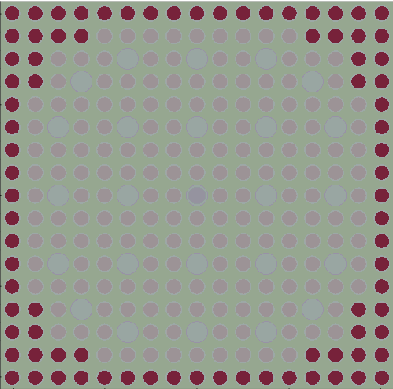
\includegraphics[width=0.9\linewidth]{figures/unsupervised/features/assm-16/u238-capt/mean-std/geometry-2}
  \caption{}
  \label{fig:chap10-capt-mean-std-geom-2}
\end{subfigure}%
\begin{subfigure}{0.45\textwidth}
  \centering
  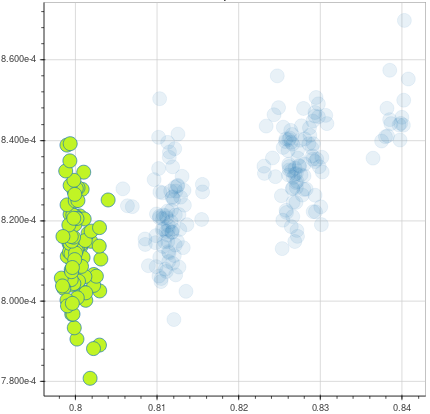
\includegraphics[width=0.9\linewidth]{figures/unsupervised/features/assm-16/u238-capt/mean-std/mgxs-2}
  \caption{}
  \label{fig:chap10-capt-mean-std-mgxs-2}
\end{subfigure}
\begin{subfigure}{0.45\textwidth}
  \centering
  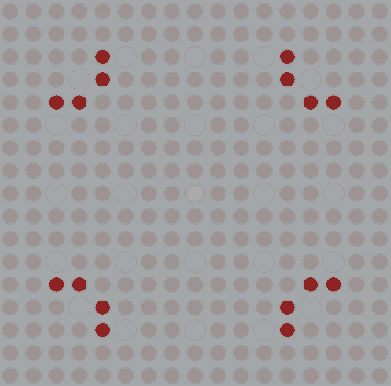
\includegraphics[width=0.9\linewidth]{figures/unsupervised/features/assm-16/u238-capt/mean-std/geometry-3}
  \caption{}
  \label{fig:chap10-capt-mean-std-geom-3}
\end{subfigure}%
\begin{subfigure}{0.45\textwidth}
  \centering
  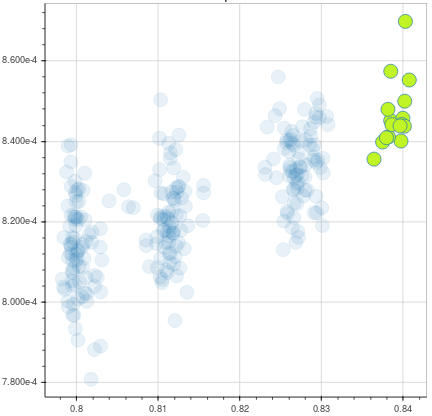
\includegraphics[width=0.9\linewidth]{figures/unsupervised/features/assm-16/u238-capt/mean-std/mgxs-3}
  \caption{}
  \label{fig:chap10-capt-mean-std-mgxs-3}
\end{subfigure}
\caption[Clustering of U-238 capture MGXS]{Scatter plots of the pin-wise U-238 capture MGXS means [barns] ($x$) and relative statistical uncertainties [\%] ($y$) in barns for a 1.6\% enriched fuel assembly.}
\label{fig:capt-mean-std}
\end{figure}

%%%%%%%%%%%%%%%%%%%%%%%%%%%%%%%%%%%%%%%%%%%%%%%%%%%%%%%%%%%%%
\subsection*{Null, Degenerate and LNS Spatial Homogenization}

This work developed several different spatial homogenization schemes to model spatial self-shielding effects in MGXS. Although all spatial zones may experience spatial self-shielding, this thesis only models the impact of spatial self-shielding on MGXS in fissile regions. Each scheme uses a single MC calculation of the complete heterogeneous geometry to collapse MGXS with the ``true'' flux. The null, LNS and degenerate schemes model spatial self-shielding for each fuel pin with increasing granularity and complexity.

\textbf{\textit{Null spatial homogenization} is the simplest method and averages all spatial self-shielding effects across the entire geometry.} Null homogenization does not account for spatial self-shielding effects experienced by different fuel pins and is equivalent to averaging the data points in Fig.~\ref{fig:capt-mean-std} to compute a single MGXS to be used in all fuel pins. \textbf{\textit{Degenerate spatial homogenization} takes the opposite approach and assigns each fuel pin its own MGXS.} The degenerate scheme accounts for the different spatial self-shielding effects experienced by each instance of each fuel pin throughout a heterogeneous geometry, and is equivalent to modeling each of the data points in Fig.~\ref{fig:capt-mean-std} as its own unique cluster. Although degenerate homogenization is more accurate than null homogenization, it requires many more MC particle histories to converge the uncertainties on the MGXS tallied separately for each fuel pin.

\textbf{\textit{LNS spatial homogenization} uses OpenCG's LNS algorithm to predict the clustering of pin-wise MGXS based on an analysis of the combinatorial geometry.} The LNS scheme is akin to \textit{geometric templates} employed by some lattice physics codes, such as CASMO~\cite{rhodes2006casmo}, to predict which groupings of pins are likely to experience similar spatial self-shielding effects and hence have similar MGXS. The LNS algorithm groups fuel pins together based on an analysis of each pin's neighbors. The MGXS are homogenized from ``noisy'' MC tally data across all pins within the same LNS grouping. LNS homogenization is an attempt to model MGXS clustering with fewer materials than degenerate homogenization in order accelerate the MC tally convergence rate by homogenizing MGXS across many pins. However, the LNS algorithm fails to predict spatial self-shielding effects in arbitrary core geometries, such as those that occur at assembly-assembly and assembly-reflector interfaces. These shortcomings motivate the need for an unsupervised approach to accurately and scalably predict MGXS clustering.

% scales poorly for large geometries and

%Pins with like neighboring pins, within assemblies with like neighboring assemblies, will receive the same LNS identifier.

%LNS homogenization computes a single set of MGXS for the fuel pin in each set classified by the LNS algorithm using a MC track density-weighted averages of the reaction rates and flux tallies in each pin.

%\begin{equation}
%\label{eqn:imgxs-micro}
%\hat{\sigma}_{x,i,m,g} = \frac{\displaystyle\sum\limits_{k=1}^{K}\mathbb{1}_{\mathbb{S}_{m}}(k) \langle \sigma_{x,i}, \psi \rangle_{k,g}^{t\ell}}{\displaystyle\sum\limits_{k=1}^{K}\mathbb{1}_{\mathbb{S}_{m}}(k) \langle \psi \rangle_{k,g}^{t\ell}}
%\end{equation}

%%%%%%%%%%%%%%%%%%%%%%%%%%%%%%%%%%%%%%%%%%%%%%%%%%%
\subsection*{\textit{i}MGXS Spatial Homogenization}

\textbf{\textit{Inferential MGXS spatial homogenization} uses machine learning to infer MGXS clusters directly from ``noisy'' MC tally data.} The \textit{i}MGXS scheme can flexibly accommodate arbitrary core heterogeneities better than heuristic approaches like LNS which must be customized for particular core geometries. In addition, the \textit{i}MGXS scheme accelerates the convergence rate of MGXS tallied with MC with respect to the degenerate and LNS schemes since it homogenizes MC tallies across many more fuel pins.

% rather than predict clustering from an analysis of the core geometry.

The \textit{i}MGXS spatial homogenization scheme is a multi-stage data processing pipeline as illustrated in Fig.~\ref{fig:imgxs-flow-chart}. The \textit{feature extraction} stage of the pipeline builds features (\textit{i.e.}, random variables) derived from ``noisy'' MC tally data which provide information about MGXS clustering for each fuel pin. The \textit{feature selection} stage removes redundant and/or highly correlated features to minimize the number of features used to train a clustering model. The \textit{dimensionality reduction} stage projects samples in a lower-dimensional vector space with the same descriptive power as the original features to reduce training time and and improve clustering model performance. The \textit{predictor training} stage builds a series of clustering models for different parameters (\textit{e.g.}, varying numbers of clusters), each of which predicts clusters of fuel pins that are grouped together with the same MGXS. The $k$-means~\cite{macqueen1967kmeans, lloyd1982kmeans}, agglomerative~\cite{johnson1967hierarchical}, BIRCH~\cite{zhang1996birch} and Gaussian Mixture Model~\cite{mclachlan1988mixture} clustering algorithms were each employed within the \textit{i}MGXS scheme for this thesis. The \textit{model selection} stage evaluates heuristics to choose clustering model parameters, including the number of clusters. Various methods which score clustering models based upon their intra- and inter-cluster similarities, or penalize model complexity using regularization, were evaluated within the \textit{i}MGXS scheme.

\begin{figure}[h!]
\centering
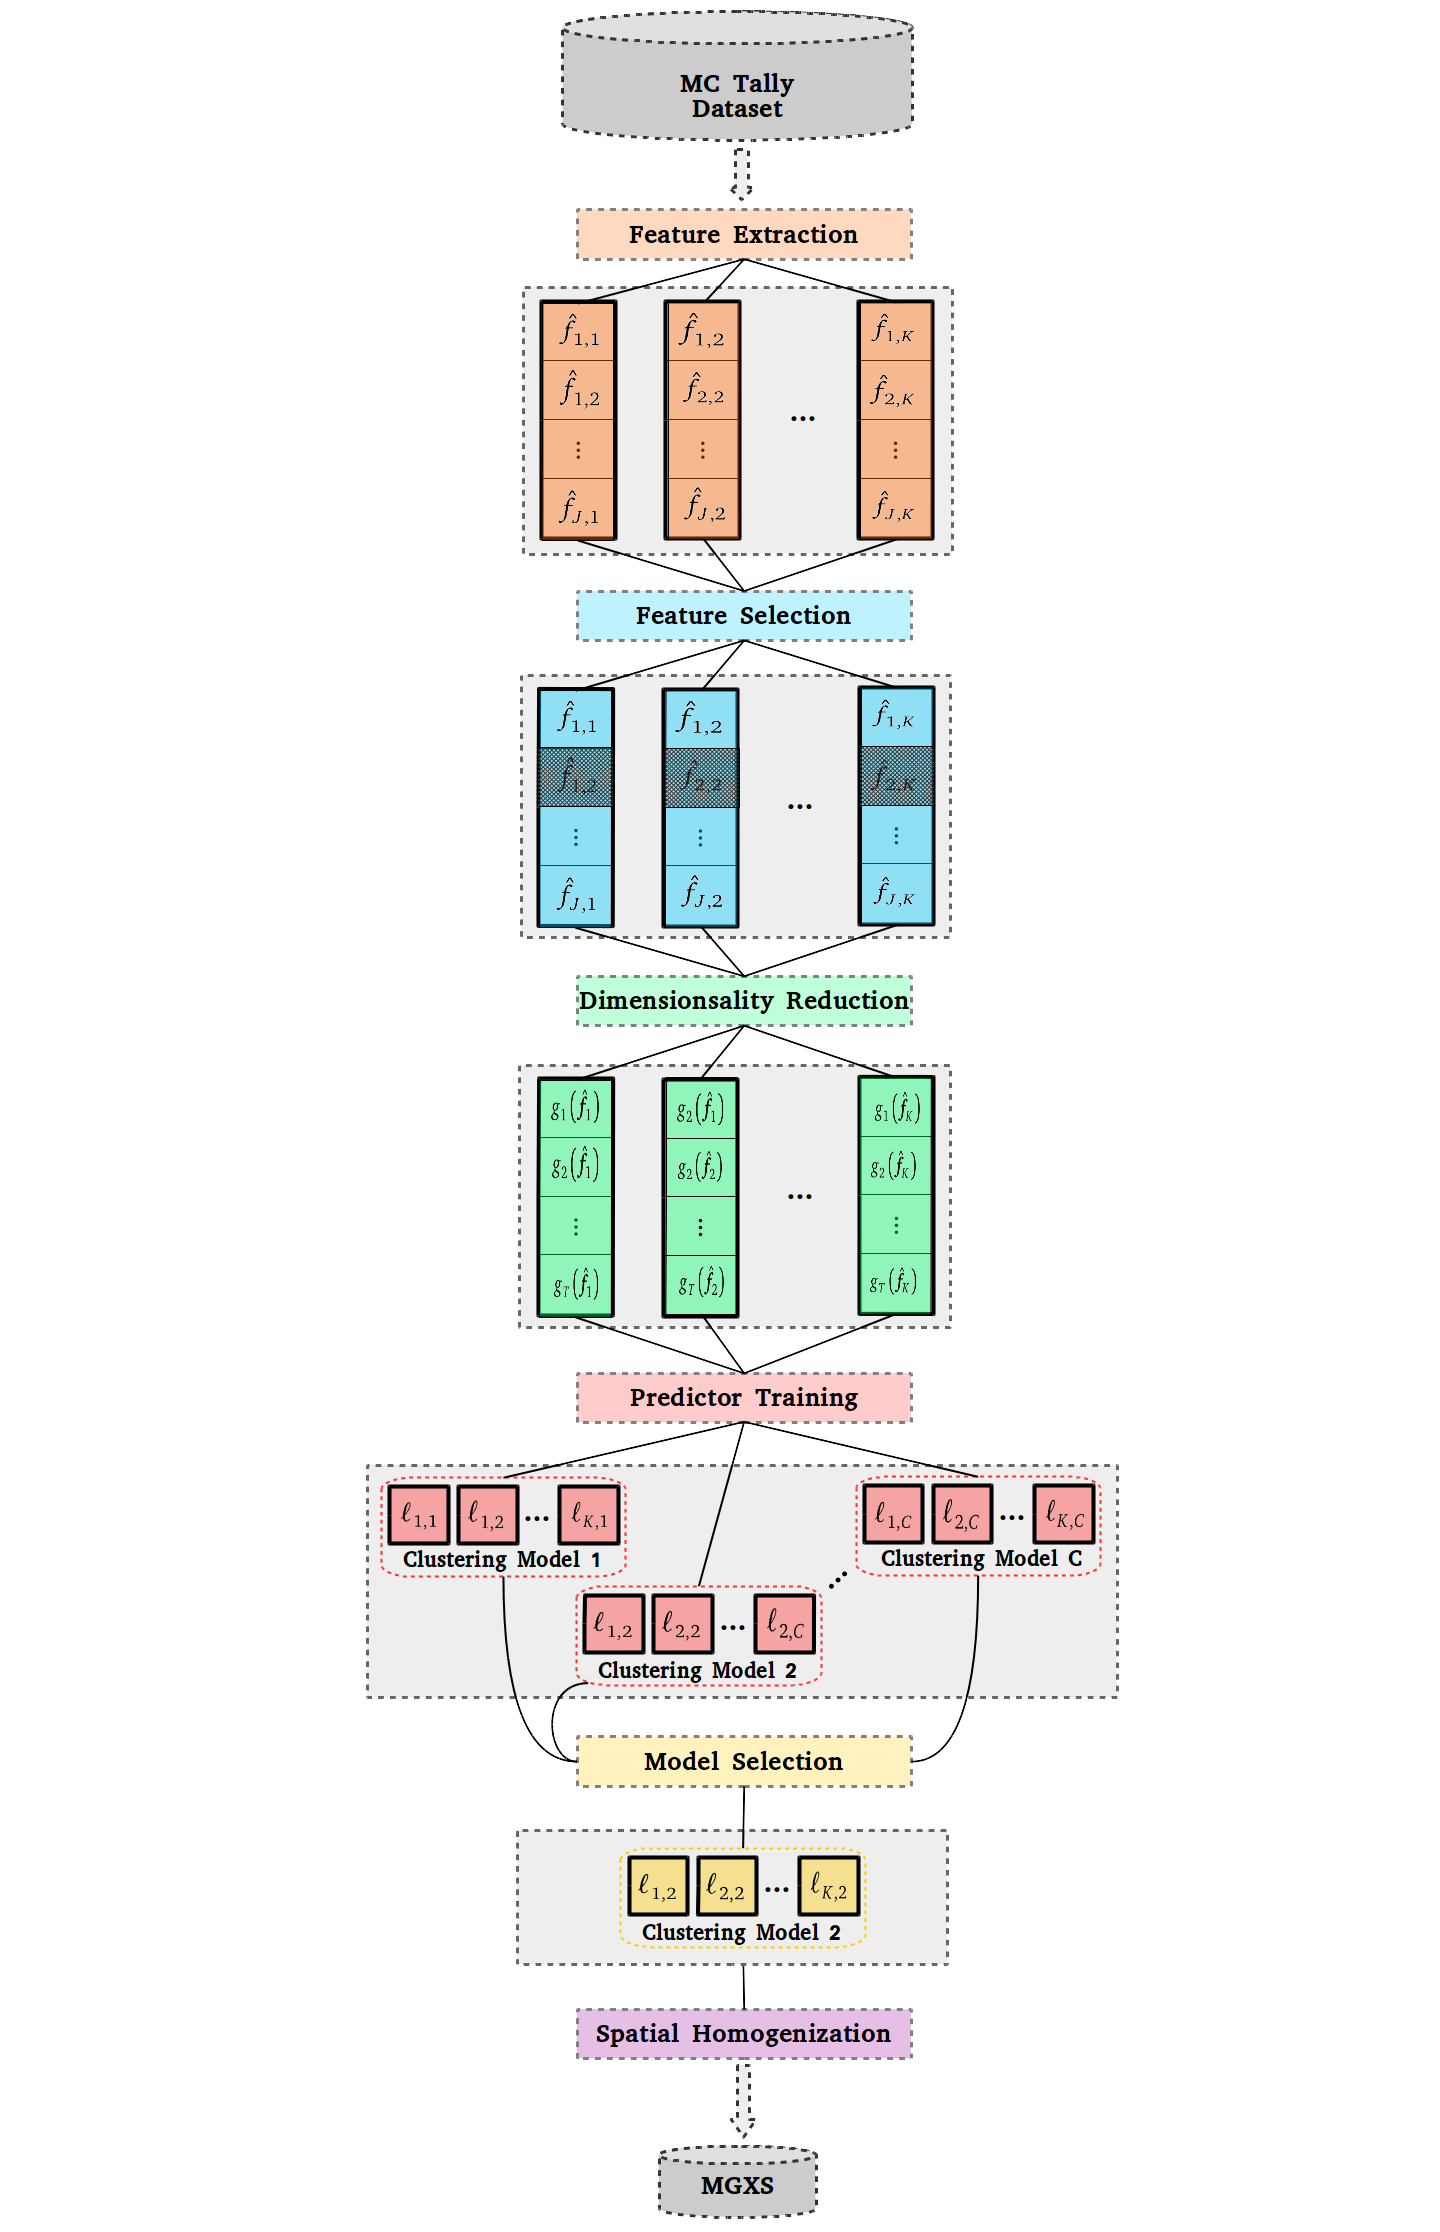
\includegraphics[width=0.88\linewidth]{figures/unsupervised/features/engineering/flow-chart}
\vspace{2mm}
\caption[\textit{i}MGXS flow chart]{The \textit{i}MGXS data processing pipeline.}
\label{fig:imgxs-flow-chart}
\end{figure}


%%%%%%%%%%%%%%%%%%%%%%%%%%%%%%%%%%%%%%%%%%%%%%%%%%%%%%%%%%%%%%%%%%%%%%%%%%%%%%%%
\section*{Model Validation}

%%%%%%%%%%%%%%%%%%%%%%%%%%%%%%%%%%%%%%%%%%
\subsection*{Heterogeneous PWR Benchmarks}

A series of six 2D heterogeneous benchmarks were derived from the Benchmark for Evaluation And Validation of Reactor Simulations (BEAVRS) Pressurized Water Reactor (PWR) model~\cite{horelik2013beavrs} to evaluate the \textit{i}MGXS scheme. BEAVRS is a highly-detailed PWR specification which was created to validate high-fidelity core analysis methods. One of the benchmarks was constructed as a 2$\times$2 ``mini core'' of 1.6\% and 3.1\% enriched fuel assemblies surrounded by a water reflector as depicted in Fig.~\ref{fig:reflector}. \textbf{The mini core was designed to quantify the impact of the moderation provided by the reflector, and the leakage of neutrons through the reflector, on spatially self-shielded MGXS.}

The most complex benchmark was a 2D planar slice of the top right quadrant of the BEAVRS model as depicted in Fig.~\ref{fig:full-core}. The quarter core model is the all rods out configuration at the core axial mid-plane with a critical boron concentration, and includes assemblies with 1.6\%, 2.4\% and 3.1\% enriched fuel as depicted in Fig.~\ref{fig:full-core}, respectively. \textbf{The BEAVRS model was designed to quantify the effects of radial heterogeneities including the inter-assembly water gaps, stainless steel baffle surrounding the fuel assemblies, core barrel and neutron shield panels on spatially self-shielded MGXS.} 

%\textbf{The benchmarks were designed with increasingly complex heterogeneous features -- and corresponding spatial self-shielding effects -- in order to understand their implications for accurate pin-wise MGXS generation.} In particular, the impact of fuel enrichment, control rod guide tubes (CRGTs), burnable poisons (BPs), inter-assembly currents, water reflectors, steel baffles and the core barrel and vessel is considered.

%Five of the six benchmark models are based upon sub-components of the full core BEAVRS model, while the sixth benchmark is of the full BEAVRS core model. 

%The space outside of the pressure vessel is filled with air with vacuum boundaries applied to the top and right with reflective booundaries on the bottom and left.
 
%The reflected mini core includes reflective boundaries on the top and left with vacuum boundaries on the bottom and right.

%The mini core benchmark includes the effects of inter-assembly spatial heterogeneities on the spatially self-shielded MGXS of fuel pins of different enrichments placed adjacent to one another. 

\begin{figure}[h!]
\centering
\begin{subfigure}{0.47\textwidth}
  \centering
  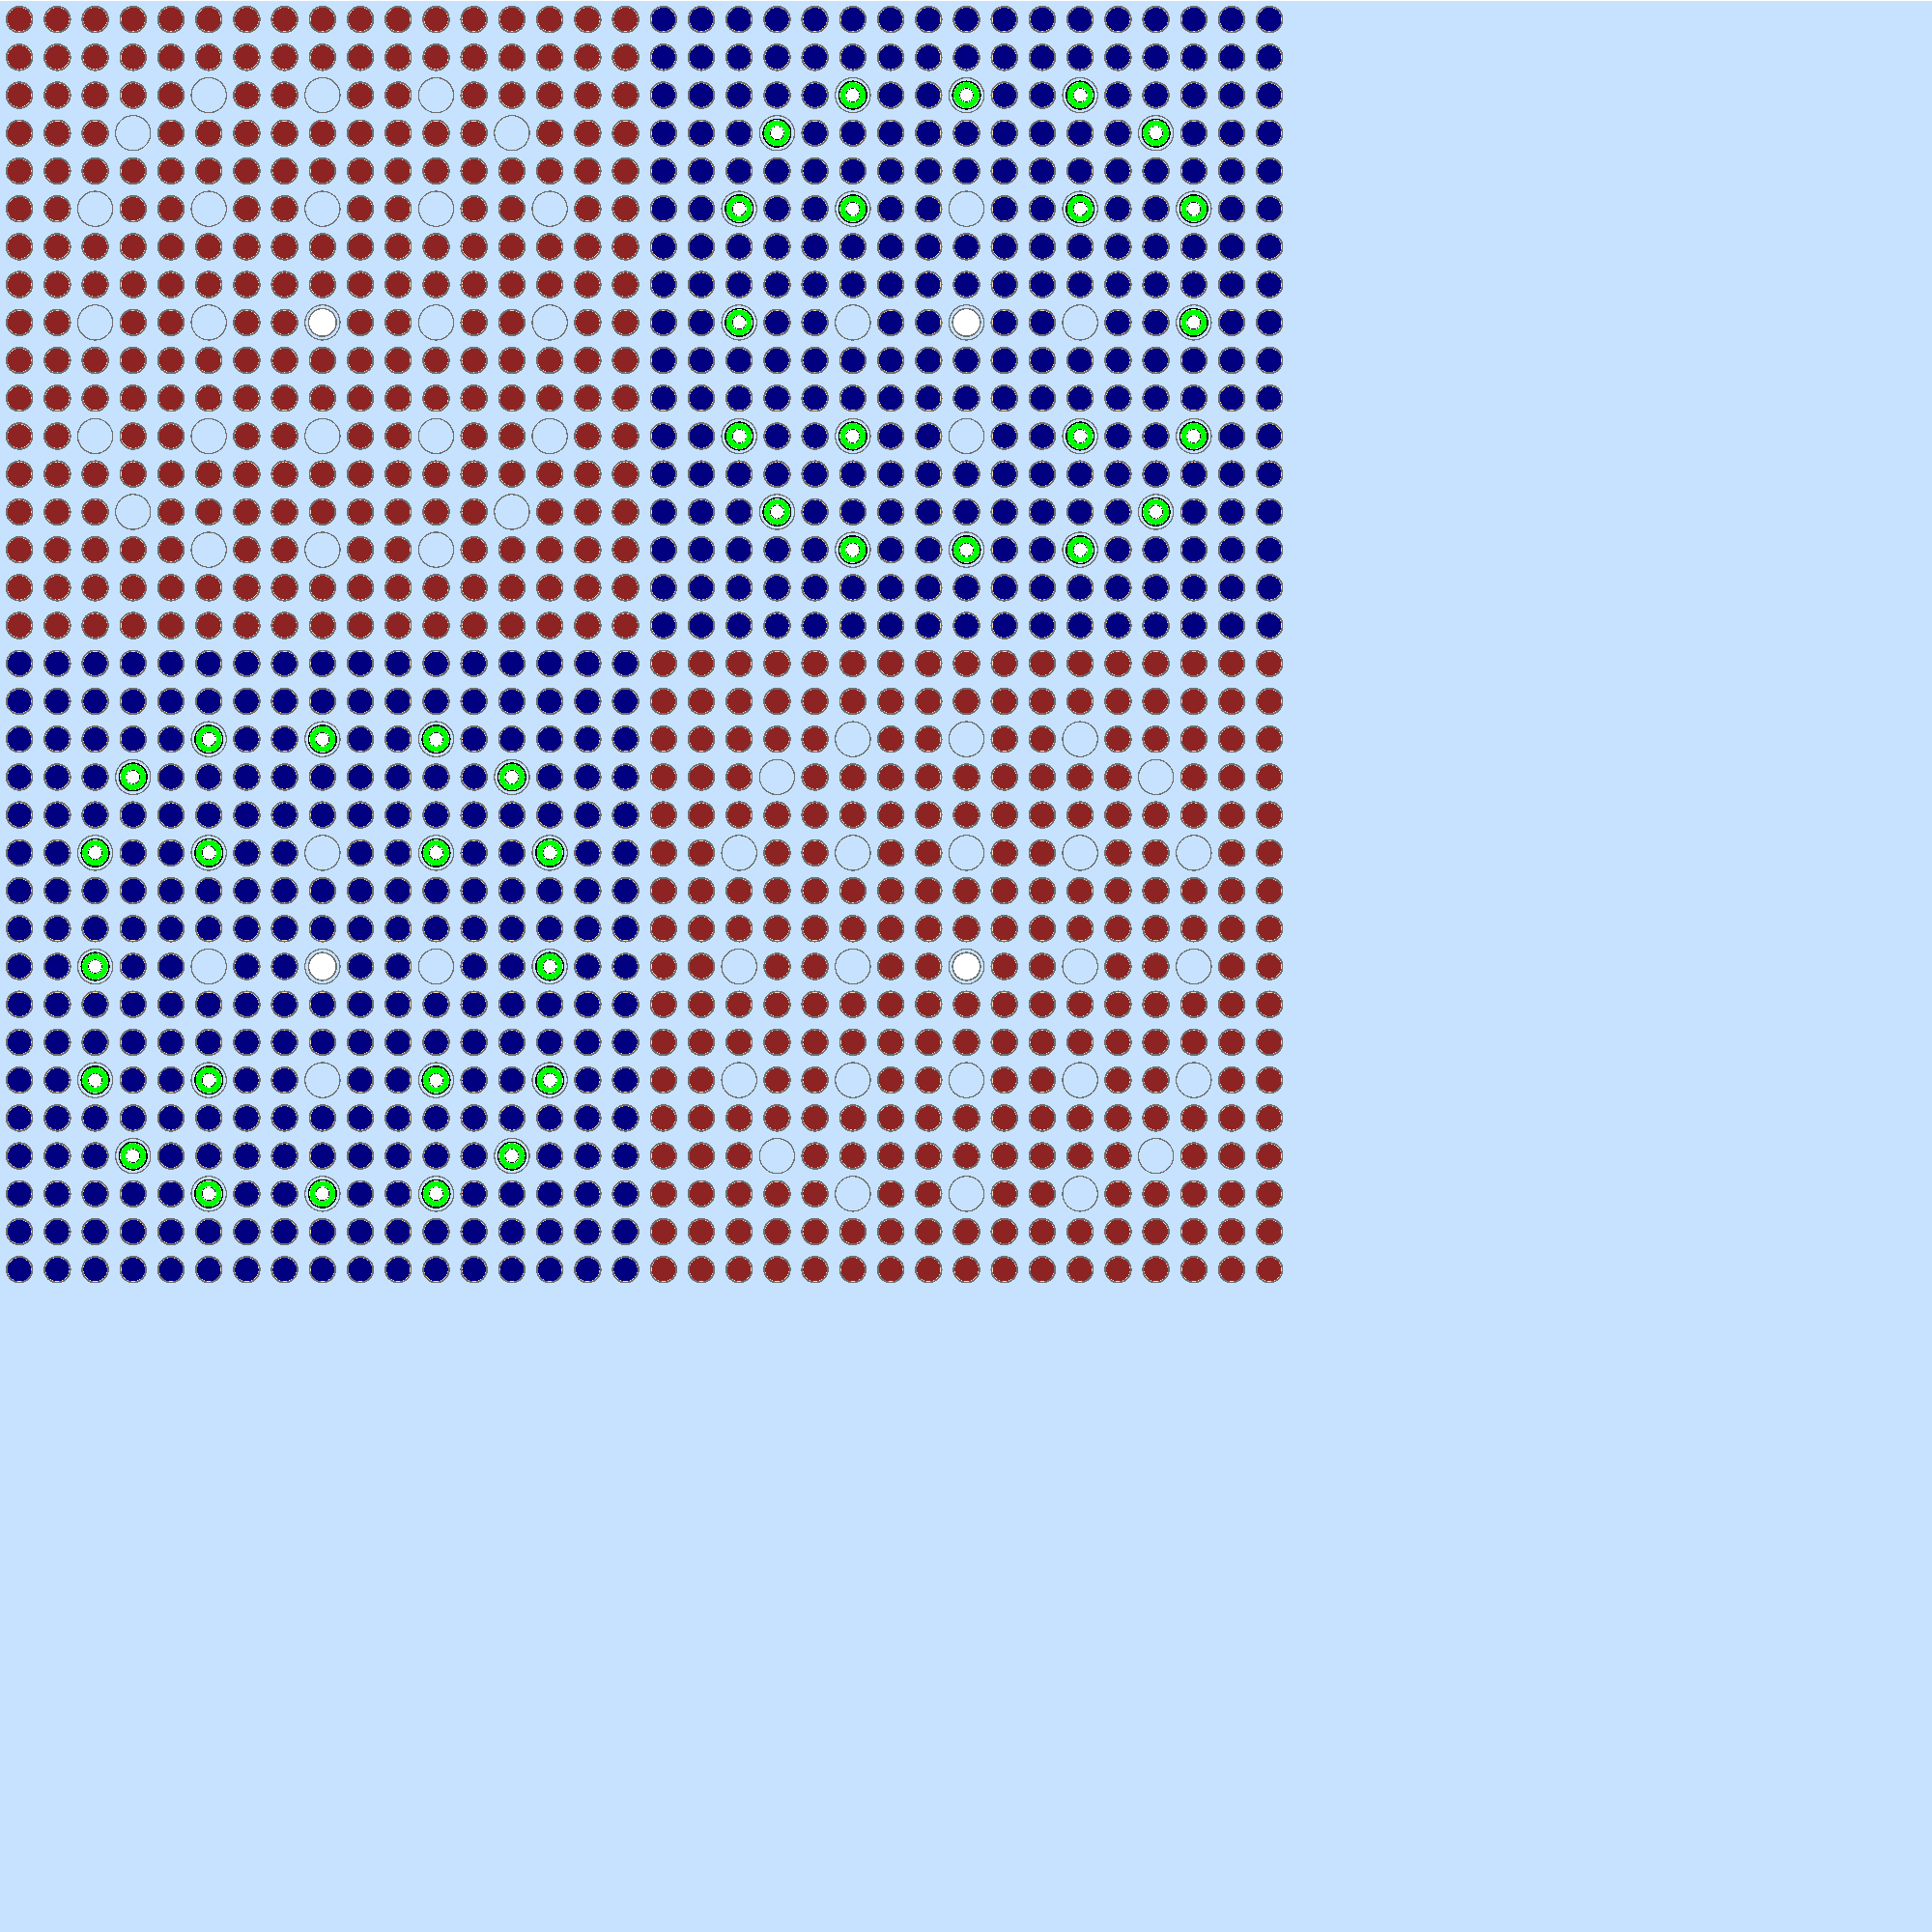
\includegraphics[width=0.93\linewidth]{figures/benchmarks/reflector}
  \caption{}
  \label{fig:reflector}
\end{subfigure}%
\begin{subfigure}{0.47\textwidth}
  \centering
  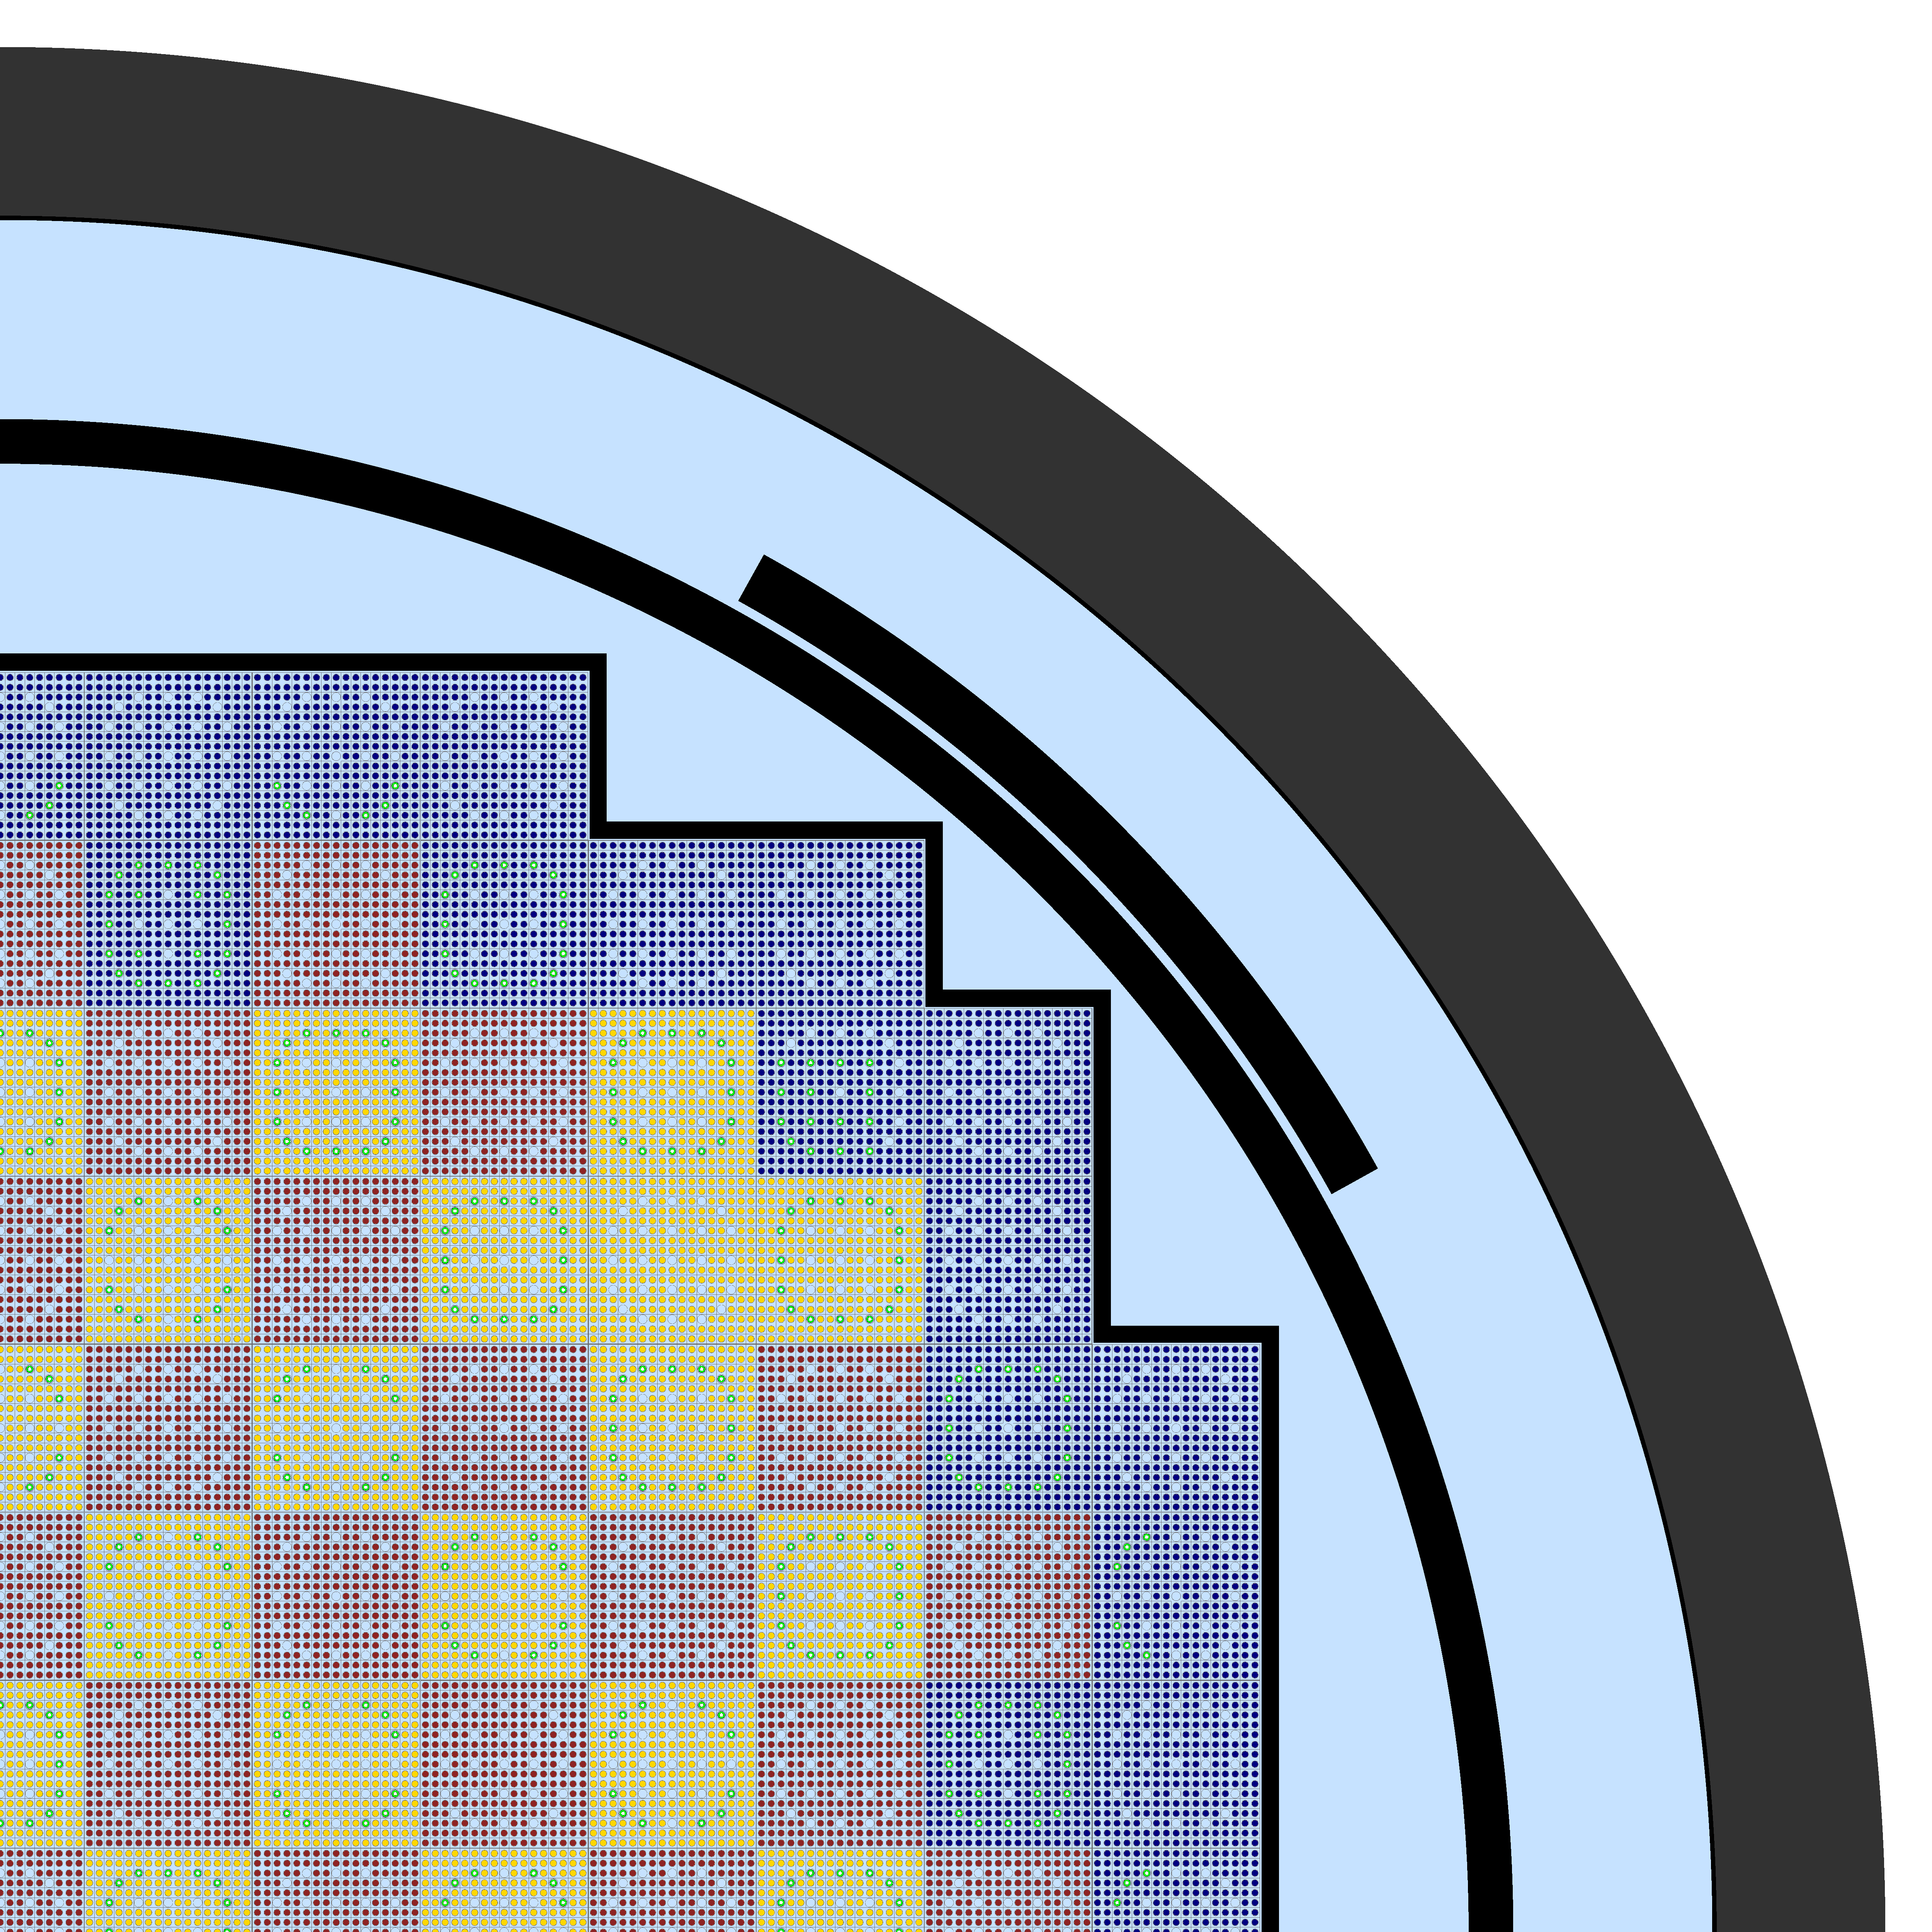
\includegraphics[width=0.93\linewidth]{figures/benchmarks/quarter-core}
  \caption{}
  \label{fig:full-core}
\end{subfigure}
\caption[PWR benchmarks]{The 2$\times$2 mini core with water reflector (a) and the quarter core BEAVRS (b) models used to evaluate the \textit{i}MGXS spatial homogenization scheme.}
\label{fig:benchmarks}
\end{figure}

%%%%%%%%%%%%%%%%%%%%%%%%%%%%%%%%%%%%%%%%%%
\subsection*{Validation Metrics}

\textbf{Each benchmark was analyzed with OpenMC to generate 70-group MGXS for use in OpenMOC. In addition, a series of OpenMC simulations calculated reference eigenvalues and pin-wise fission and U-238 capture rates for each benchmark.} The eigenvalue (\textit{i.e.}, neutron multiplication factor) is a key integral quantity used to assess the reactivity of a reactor. The fission rates are directly related to the relative power density of each fuel pin which is important for fuel depletion and thermal hydraulic feedback. The U-238 capture rates result in the production of Pu-239 which contributes up to 40\% of the power produced from fission in PWRs at the end-of-life (EOL). Hence, the spatial distributions of the fission rates and U-238 capture rates must be correctly modeled for accurate high-fidelity depletion calculations. 

\textbf{The differences in eigenvalue, fission rate and capture rates between OpenMC and OpenMOC were quantified for each benchmark and homogenization scheme.} The type of spatial homogenization strongly impacts the resultant accuracy of OpenMOC's U-238 capture rate predictions. The U-238 reaction rates display some of the largest spatial self-shielding effects -- varying by a factor of $\sim$20 between the center and outer rim of individual fuel pins -- and are especially sensitive to the spatial homogenization scheme used to generate MGXS for each pin. In contrast, the homogenization schemes have little impact on the OpenMOC fission rate predictions. As expected, the various schemes are inconsequential to the eigenvalue predictions, since each method uses the same MC flux to collapse the MGXS and preserve global reactivity. Hence, only the U-238 capture rate errors are presented and analyzed in the following section, while the eigenvalues and fission rates are reported for each benchmark in the thesis.

% This underscores the importance of accounting for spatial heterogeneities -- such as the moderation from CRGTs and reflectors -- when generating MGXS to predict U-238 capture and Pu-239 production in LWRs.

%%%%%%%%%%%%%%%%%%%%%%%%%%%
\section*{Results}

%%%%%%%%%%%%%%%%%%%%%%%%%%%%%%%%%%%%%%%%%%%%%%%%%
\subsection*{Clustered Geometries}

The geometries produced with null, degenerate, LNS and \textit{i}MGXS spatial homogenization for the 2$\times$2 mini core benchmark are displayed in Fig.~\ref{fig:colorset-geometries}. Each uniquely colored material represents a unique set of MGXS. The null scheme uses a single MGXS for each fuel pin of a particular enrichment, while the degenerate scheme assigns a unique MGXS to each fuel pin. The LNS and \textit{i}MGXS schemes distinguish fuel pins based on neighboring heterogeneities, such as control rod guide tubes and burnable poisons. Unlike LNS, the \textit{i}MGXS scheme discriminates pins along assembly-assembly and reflector-assembly interfaces. \textbf{The ability of \textit{i}MGXS to separate out fuel pins along interfaces without geometric heuristics illustrates one key advantage of \textit{i}MGXS over the LNS scheme.}

%As a result, the \textit{i}MGXS scheme is expected to outperform LNS spatial homogenization for arbitrary core geometries.

\begin{figure}[h!]
\centering
\begin{subfigure}{0.47\textwidth}
  \centering
  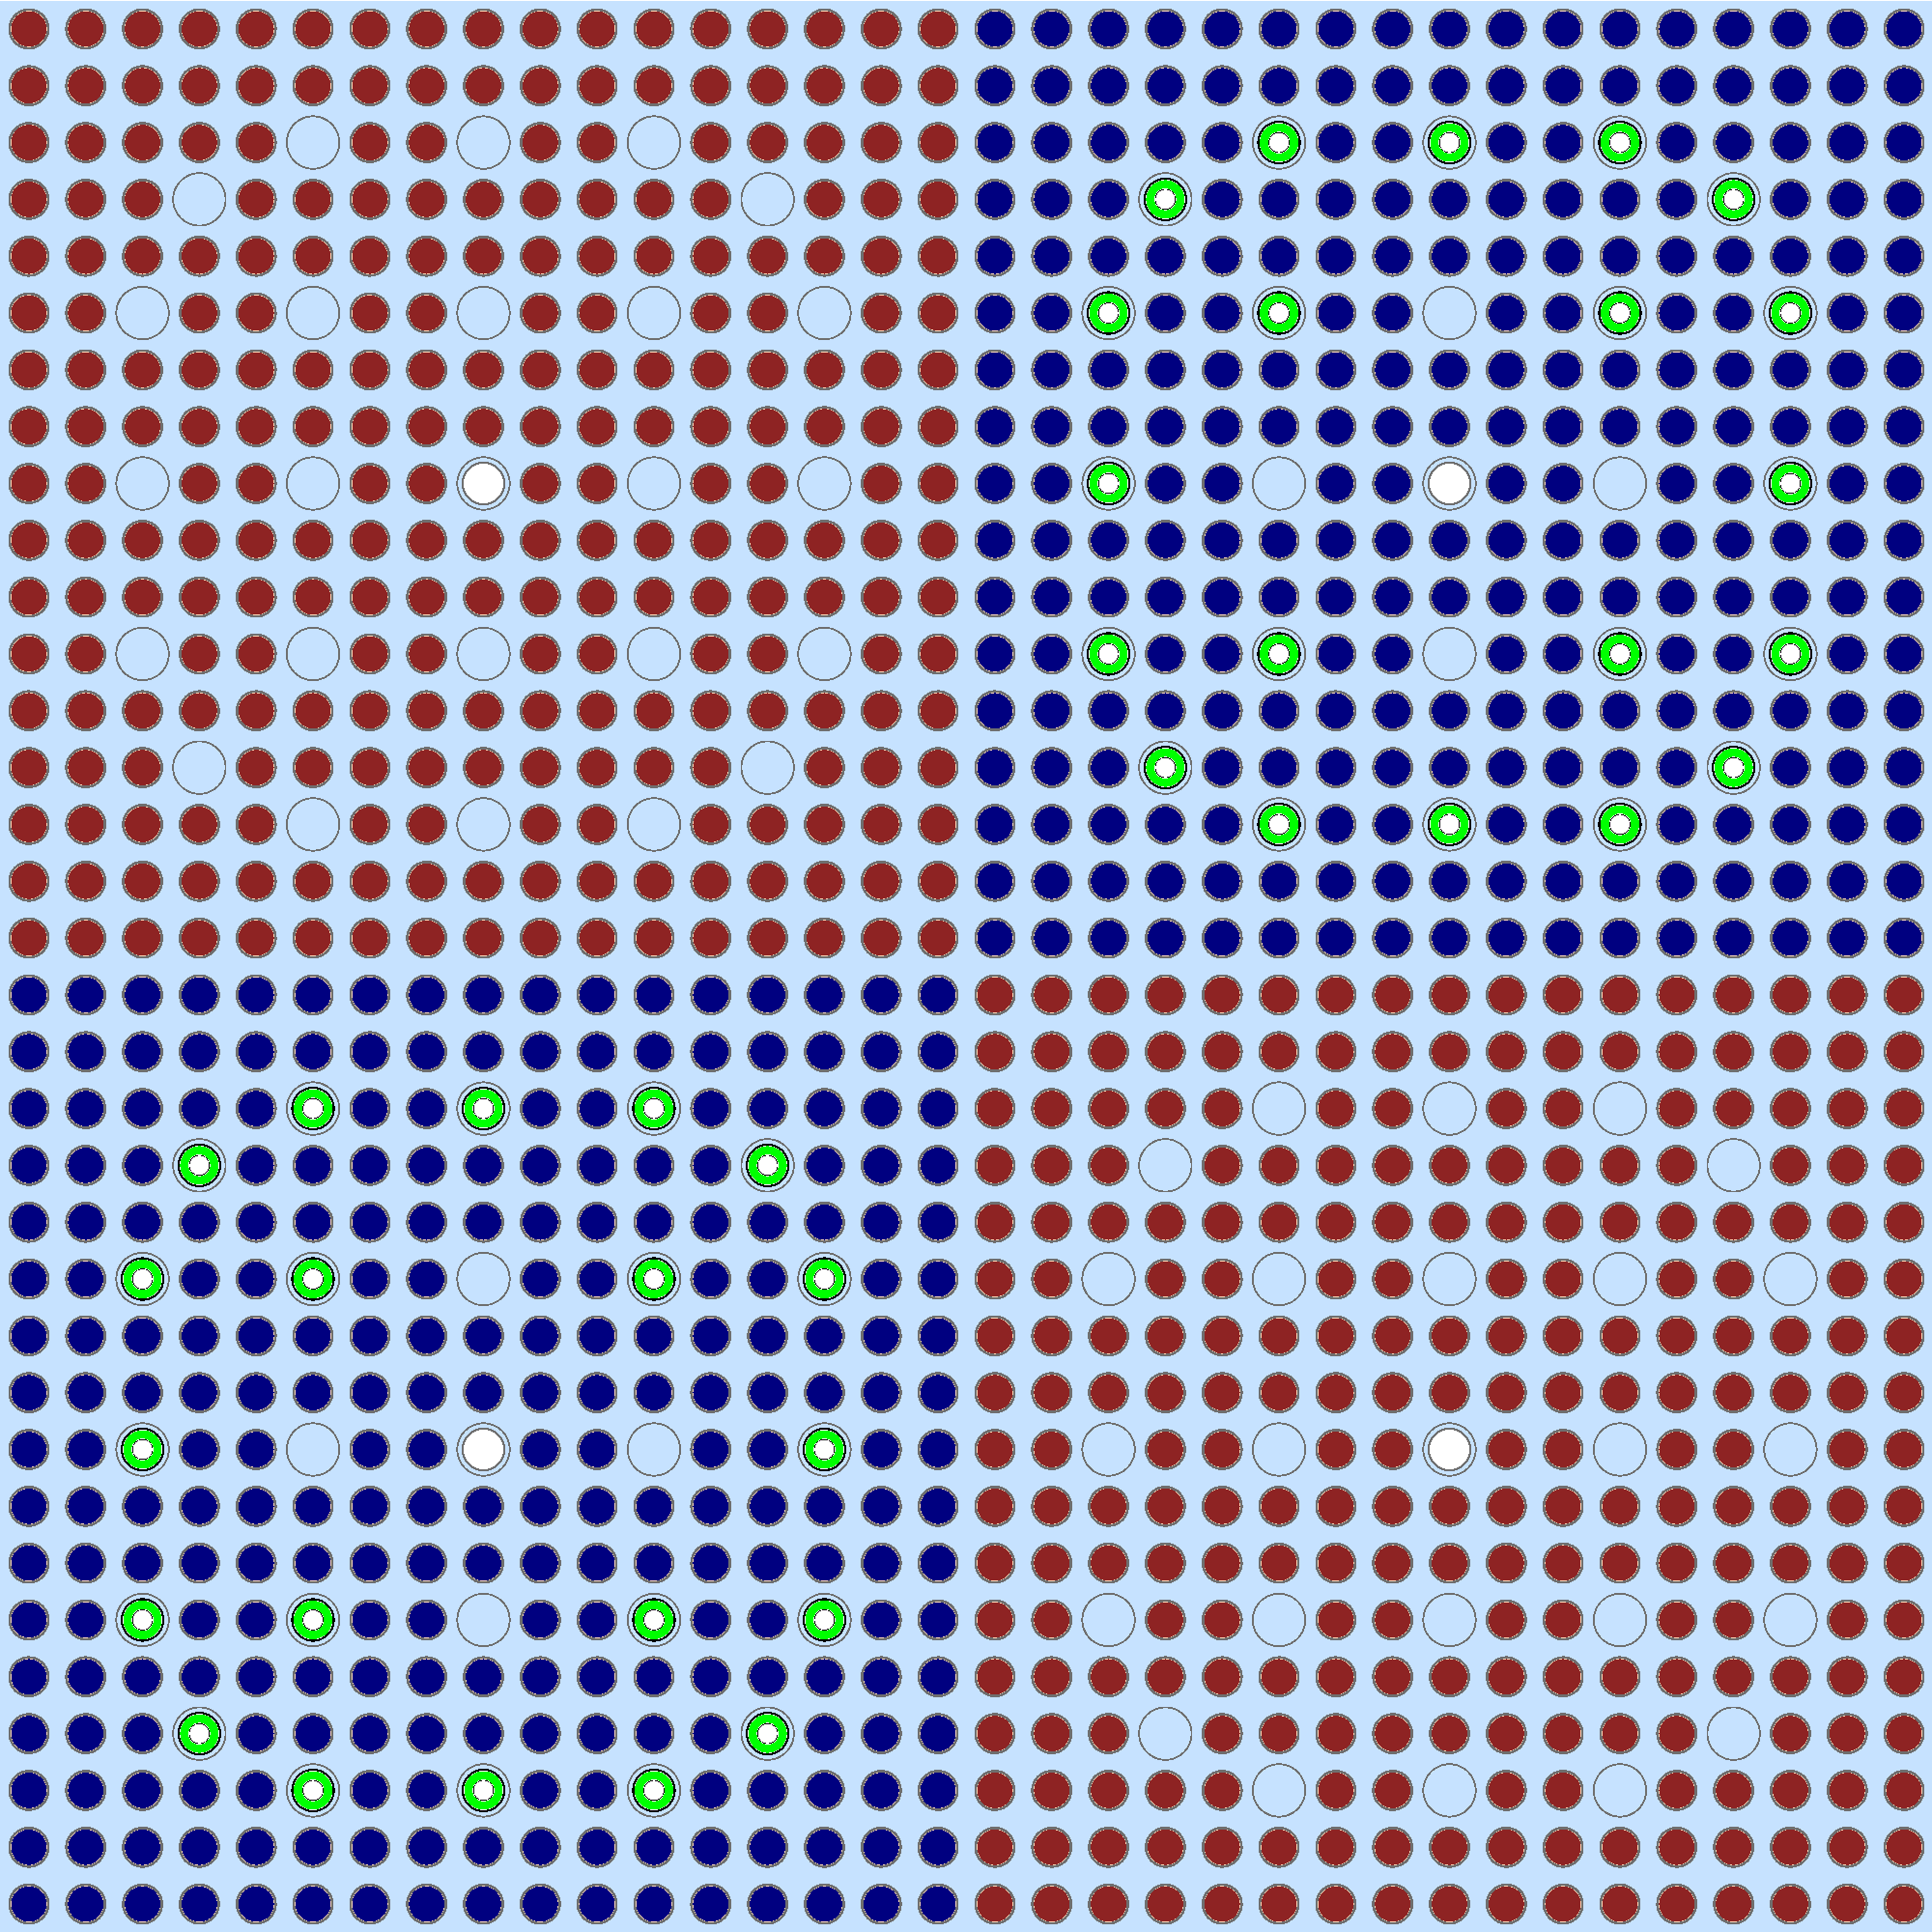
\includegraphics[width=0.75\linewidth]{figures/benchmarks/2x2}
  \caption{}
  \label{fig:reflector}
\end{subfigure}%
\begin{subfigure}{0.47\textwidth}
  \centering
  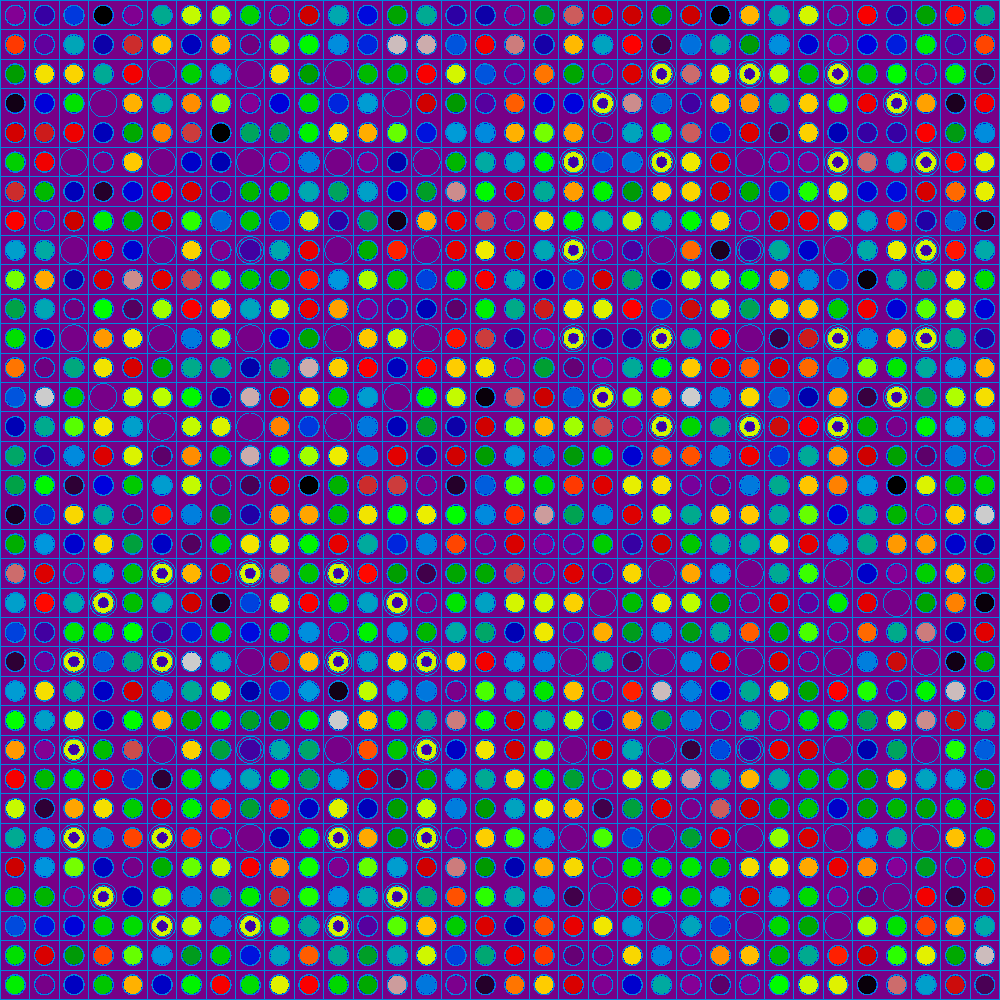
\includegraphics[width=0.75\linewidth]{figures/quantification/homogenization/2x2-degenerate-materials}
  \caption{}
  \label{fig:reflector-degenerate}
\end{subfigure}
\begin{subfigure}{0.47\textwidth}
  \centering
  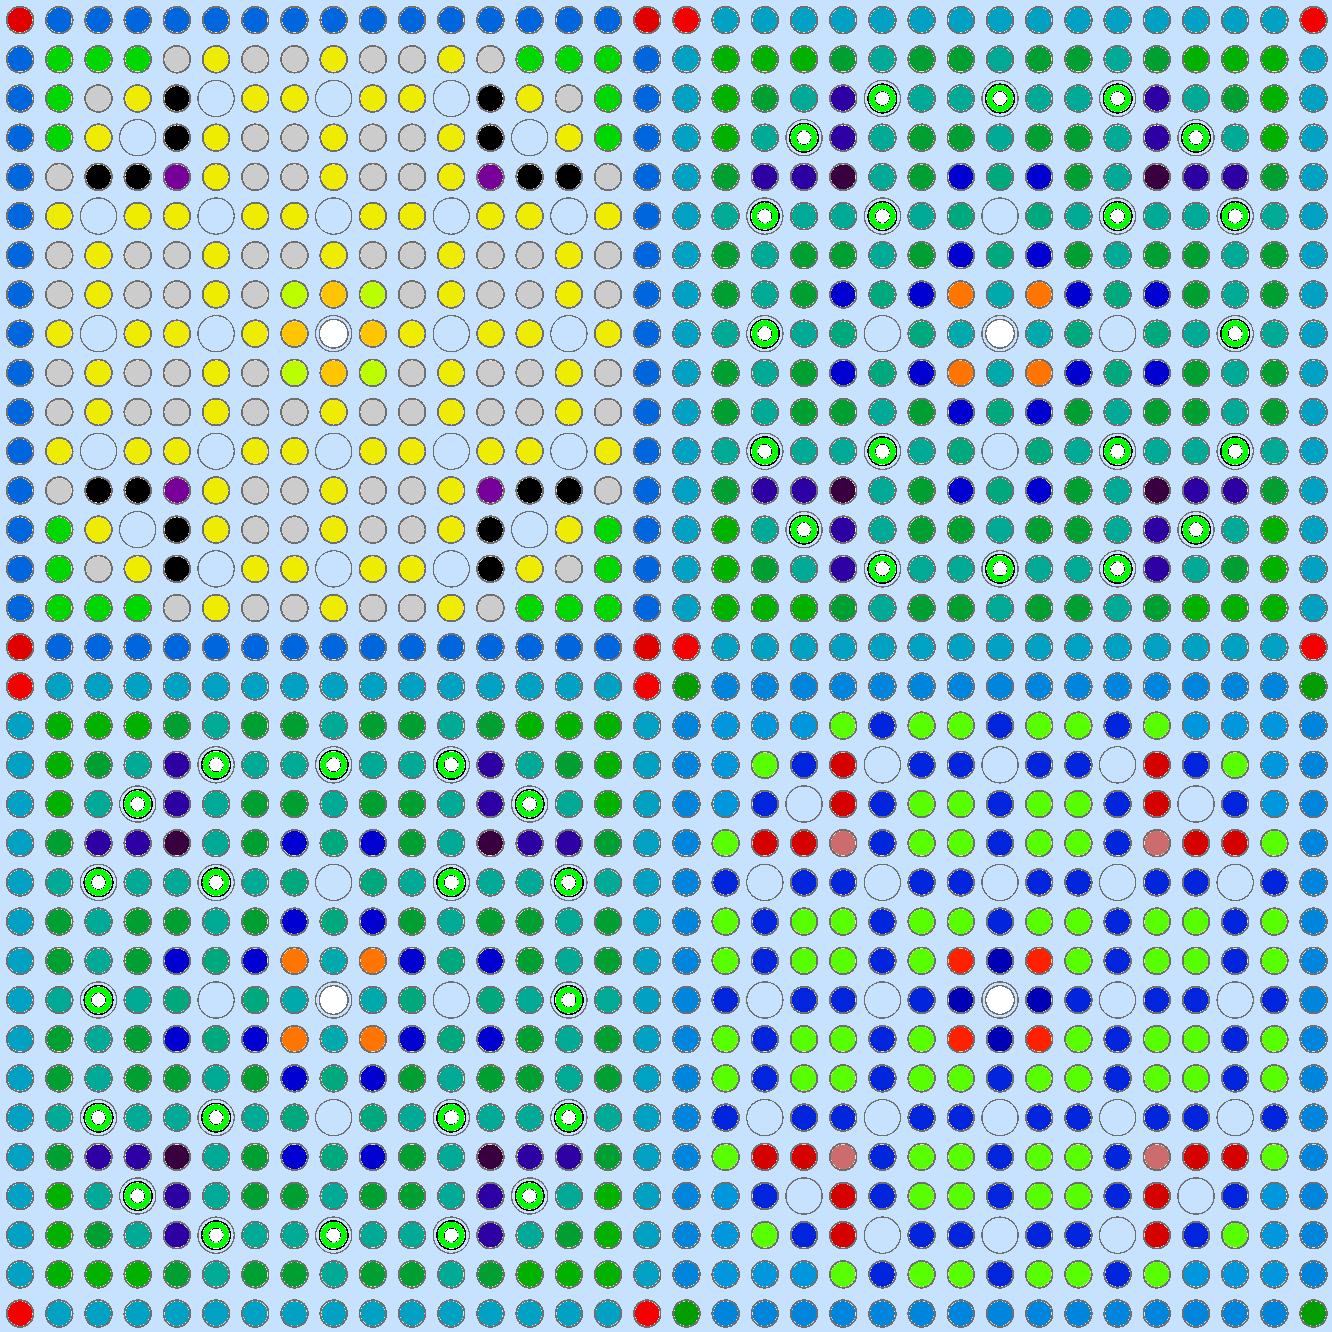
\includegraphics[width=0.75\linewidth]{figures/patterns/lns/reflector/materials}
  \caption{}
  \label{fig:reflector-lns}
\end{subfigure}%
\begin{subfigure}{0.47\textwidth}
  \centering
  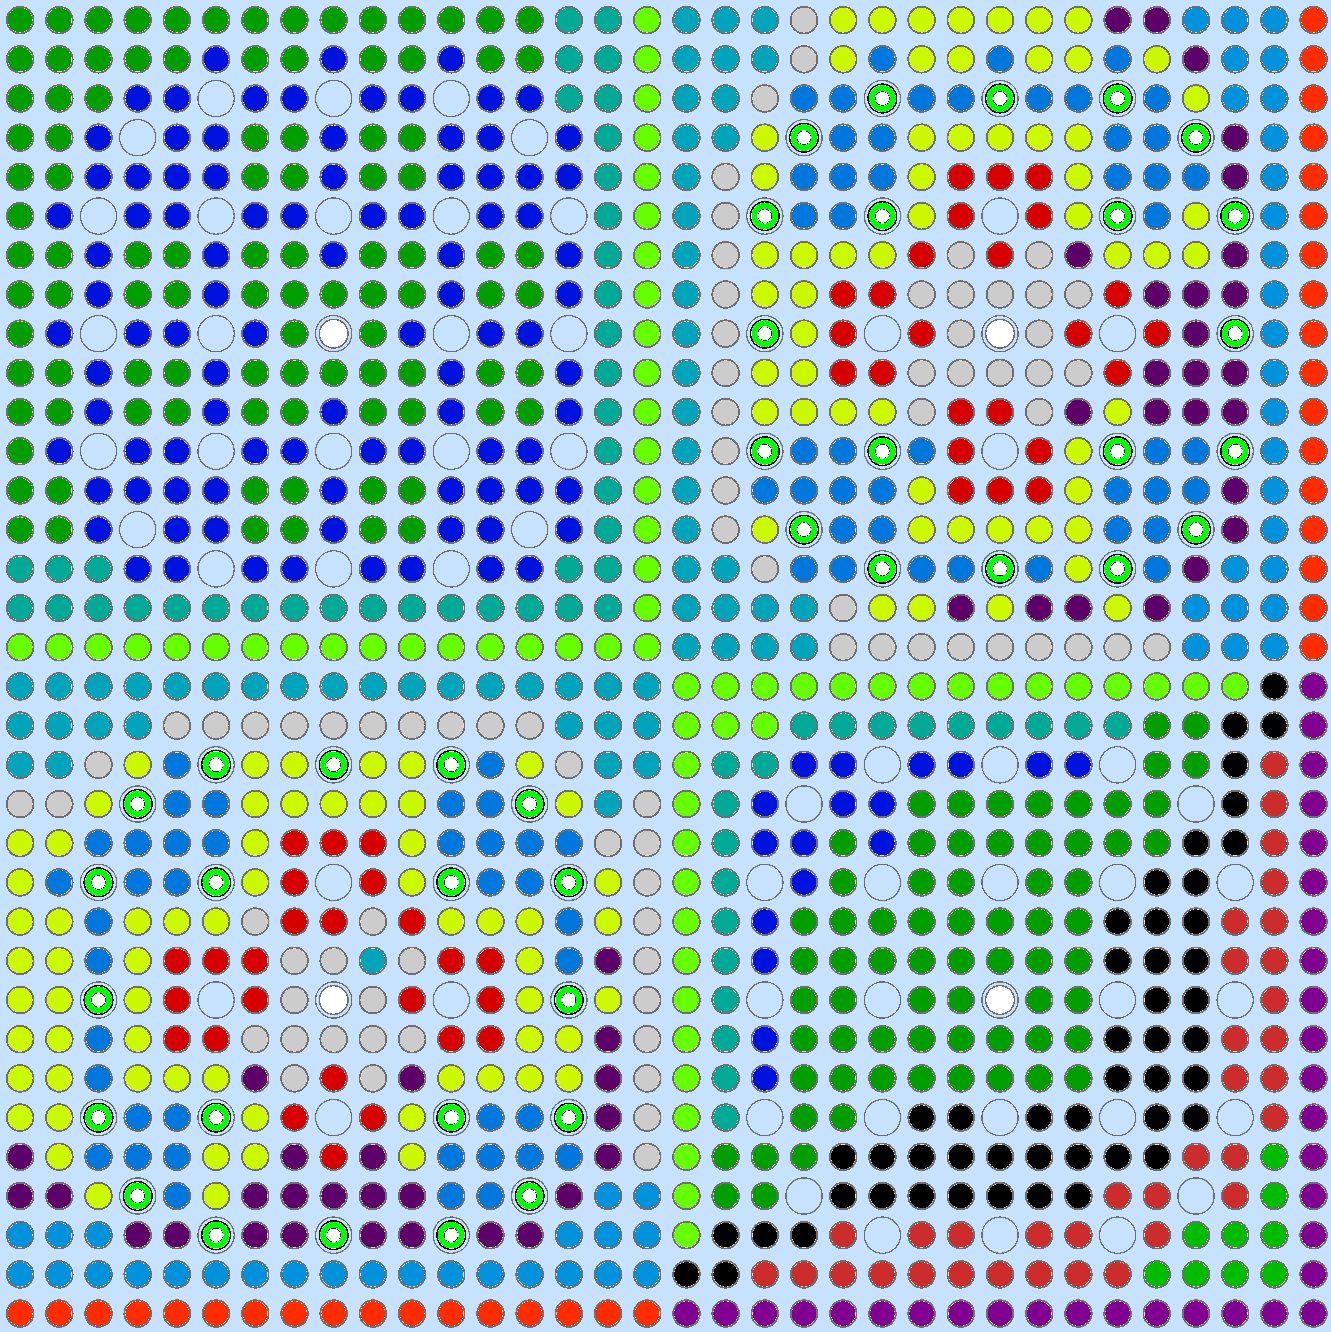
\includegraphics[width=0.75\linewidth]{figures/unsupervised/geometries/with-features/8-clusters/combined/reflector}
  \caption{}
  \label{fig:reflector-8-clusters}
\end{subfigure}
\caption[Materials for the 2$\times$2 mini core]{The materials for the 2$\times$2 mini core with null (a), degenerate (b), LNS (c) and \textit{i}MGXS spatial homogenization with 8 clusters (d).}
\label{fig:colorset-geometries}
\end{figure}

\begin{figure}[h!]
\centering
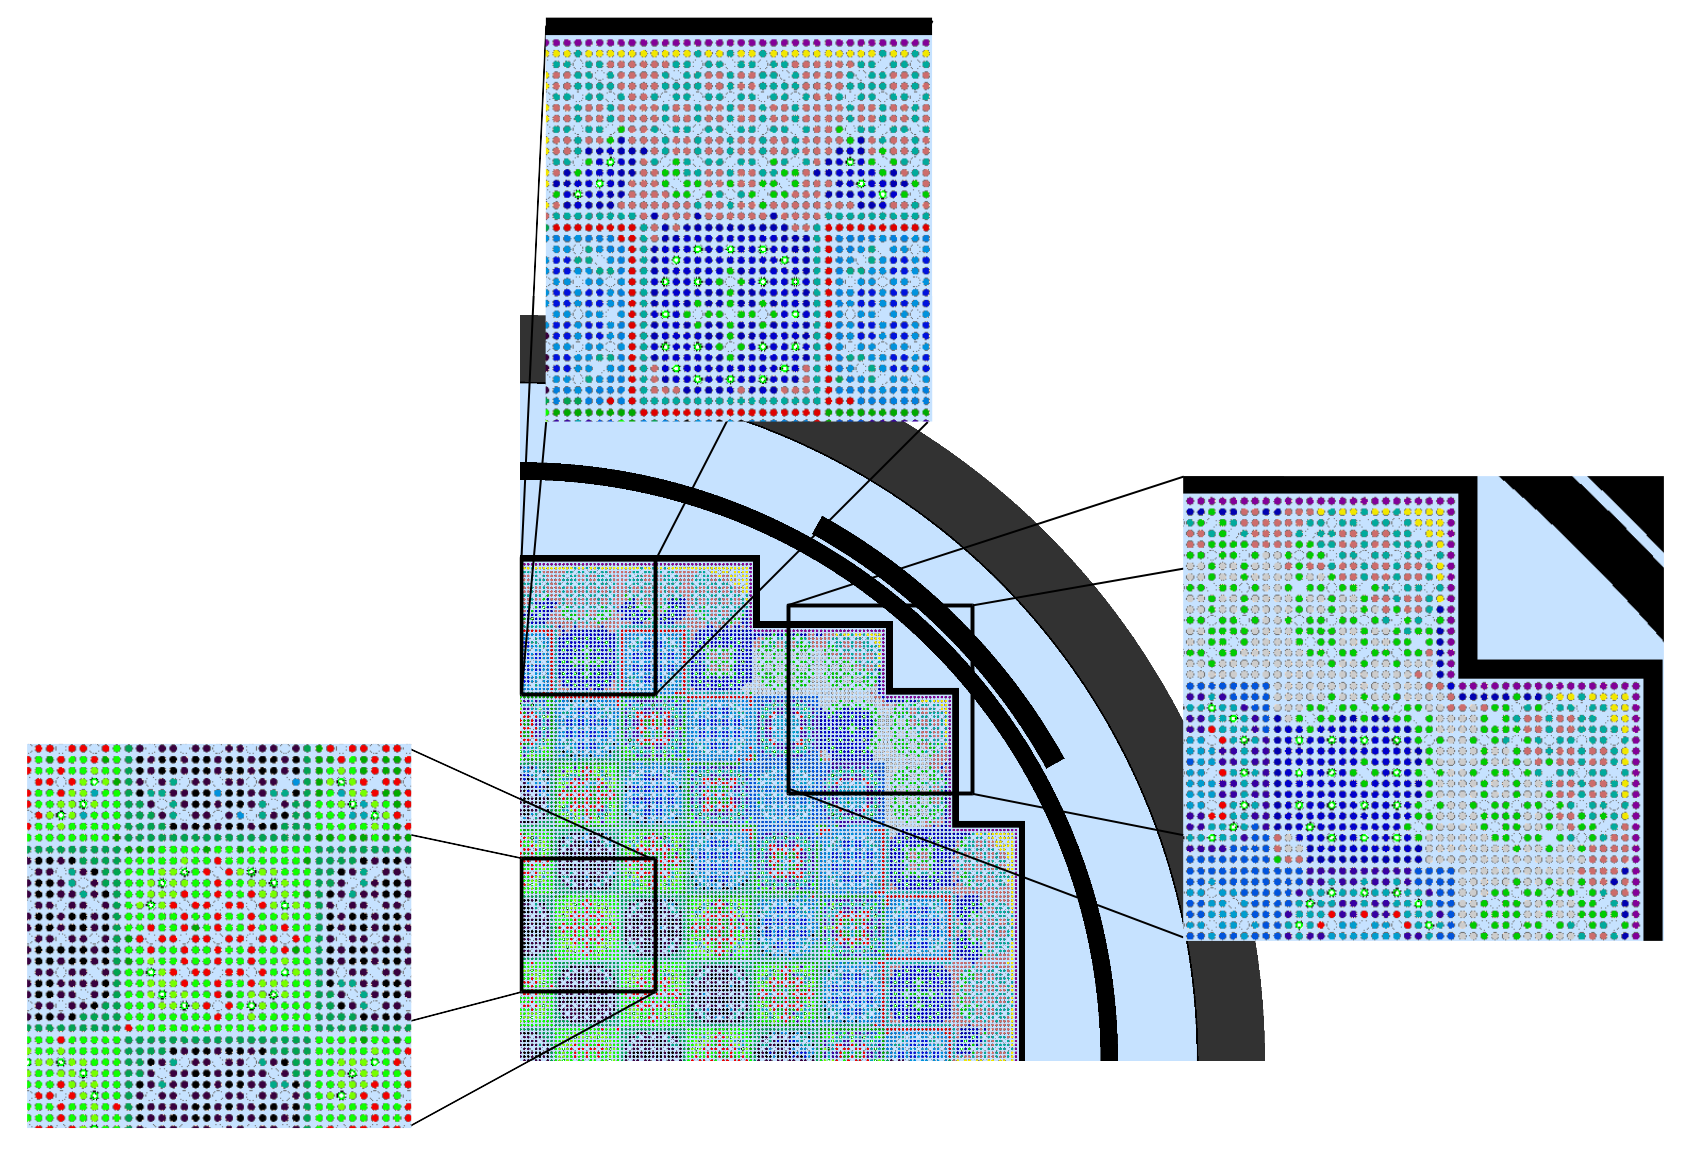
\includegraphics[width=\linewidth]{figures/unsupervised/geometries/with-features/8-clusters/combined/full-core-zoom}
\caption[Materials for the BEAVRS]{The quarter core BEAVRS model with \textit{i}MGXS spatial homogenization.}
\label{fig:full-core-8-clusters}
\end{figure}

The BEAVRS geometry built by \textit{i}MGXS with 24 clusters is presented in Fig.~\ref{fig:full-core-8-clusters}. Three zones are highlighted to illustrate the distinct clustering patterns found for interior fuel assemblies, fuel assemblies along the top baffle/reflector interface, and fuel assemblies at the corner of geometry. The pins in the interior assemblies are clustered in a way which resembles the clustered geometries found for fuel assemblies in an infinite lattice. As noted for the mini core, the \textit{i}MGXS scheme discriminates pins along assembly-assembly and reflector-assembly interfaces. Furthermore, the pins in the corner assemblies cluster according to varying levels of moderation provided by the reflector in this region of the core. These results illustrate the ability of the \textit{i}MGXS scheme to categorize fuel pins into clusters based on subtle differences in spatial self-shielding effects.

%%%%%%%%%%%%%%%%%%%%%%%%%
%\subsection*{Eigenvalues}
%
%\begin{table}[ht!]
%  \centering
%  \caption[OpenMOC eigenvalue bias]{OpenMOC eigenvalue bias $\Delta\rho$ for \textit{i}MGXS spatial homogenization.}
%  \small
%  \label{table:eigenvalues}
%  \vspace{6pt}
%  \begin{tabular}{p{4cm} R{0.9cm} R{0.9cm} R{0.9cm} R{0.9cm} R{0.9cm} R{0.9cm}}
%  \toprule
%  & \multicolumn{6}{S[table-format=6.1]}{\textbf{\# Clusters}} \\
%  \cline{2-7}
%  \multirow{-2}{*}{\bf Benchmark} &
%  \multicolumn{1}{c}{\textbf{1}} & 
%  \multicolumn{1}{c}{\textbf{2}} & 
%  \multicolumn{1}{c}{\textbf{4}} & 
%  \multicolumn{1}{c}{\textbf{8}} & 
%  \multicolumn{1}{c}{\textbf{16}} & 
%  \multicolumn{1}{c}{\textbf{\# pins}} \\
%  \midrule
%Colorset w/ Reflector & -141 & -136 & -136 & -134 & -129 & -141 \\
%  \midrule
%BEAVRS Quarter Core & -122 & -119 & -120 & -119 & -119 & -116 \\
%  \bottomrule
%\end{tabular}
%\end{table}

%%%%%%%%%%%%%%%%%%%%%%%%%%%%%%%%%%%%%%%%%%%%%%%%
\subsection*{Pin-Wise U-238 Capture Rates}

The OpenMOC energy-integrated pin-wise U-238 capture rates were compared to the reference OpenMC capture rates for each homogenization scheme to compute the percent relative errors for each pin's capture rates. The spatial distributions of capture rate errors are plotted as heatmaps for the mini core benchmark in Fig.~\ref{fig:refl-capt-err} with null, degenerate, LNS and \textit{i}MGXS homogenization with BIRCH clustering of 2, 4 and 16 clusters.

\begin{figure}[h!]
\centering
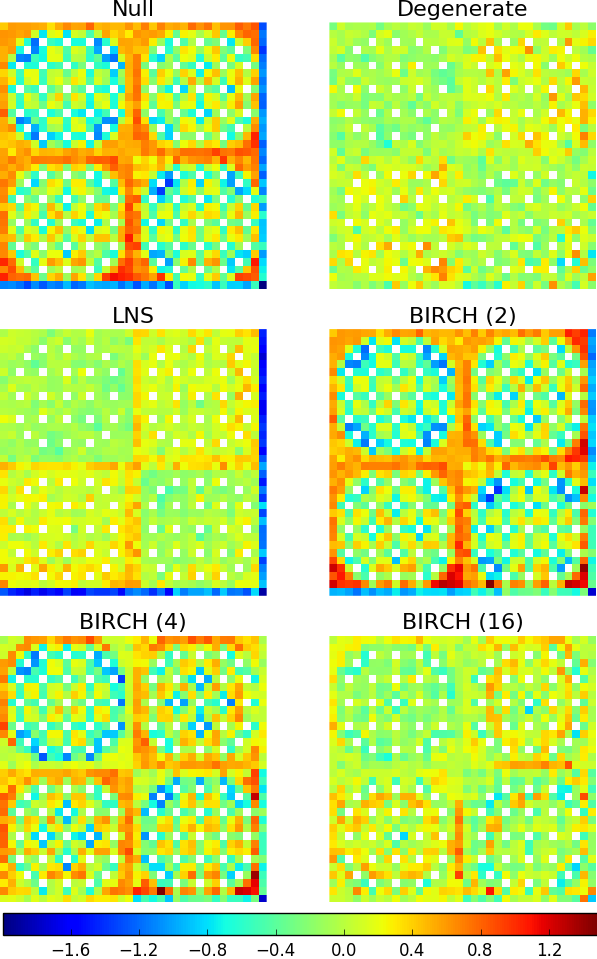
\includegraphics[width=0.83\linewidth]{figures/results/spatial/reflector/capt-err}
\vspace{2mm}
\caption[U-238 capture rate errors for the 2$\times$2 mini core]{U-238 capture rate percentage relative errors for the 2$\times$2 mini core with null, degenerate, LNS and \textit{i}MGXS spatial homogenization with 2, 8 and 16 clusters.}
\label{fig:refl-capt-err}
\end{figure}

The error is largest for the null homogenization scheme since it neglects to model MGXS clustering due to spatial self-shielding effects in each fuel pin. The error is smallest for the degenerate scheme since it exactly models the different spatial self-shielding effects for each fuel pin in the geometry. The LNS scheme largely ``smooths'' the error distribution for the interior pins, but exhibits large errors for the single outermost row of pins adjacent to the reflector, and to a lesser extent, the pins along the inter-assembly interfaces. This illustrates LNS' inability to distinguish fuel pins along interfaces between spatial zones. Unlike the LNS scheme, the \textit{i}MGXS scheme excels at discriminating pins along assembly-assembly and assembly-reflector interfaces into unique clusters such that little residual error is observed with 16 clusters.

In addition, it is often useful to compare the reaction rates from two different OpenMOC simulations with null and \textit{i}MGXS homogenization. The percent relative deviation of the U-238 capture rate distributions between the null and \textit{i}MGXS schemes can be computed to visualize the impact of clusters on the U-238 capture rate predictions. Fig.~\ref{fig:refl-capt-rates-comp} present the percent relative deviations for the mini core benchmark with BIRCH clustering of 2, 4, 8 and 16 clusters. The figures illustrate the \textit{hierarchical} nature of MGXS clustering by discriminating fuel pins with different spatial self-shielding effects that occur in different spatial regimes. For example, the first 2 -- 4 clusters discriminate pins along the assembly-assembly and assembly-reflector interfaces. As more clusters are introduced, they are increasingly customized to model the more local spatial self-shielding effects affecting the pins within the interior of each assembly due to the presence of control rod guide tubes and burnable poisons.

\begin{figure}[h!]
\centering
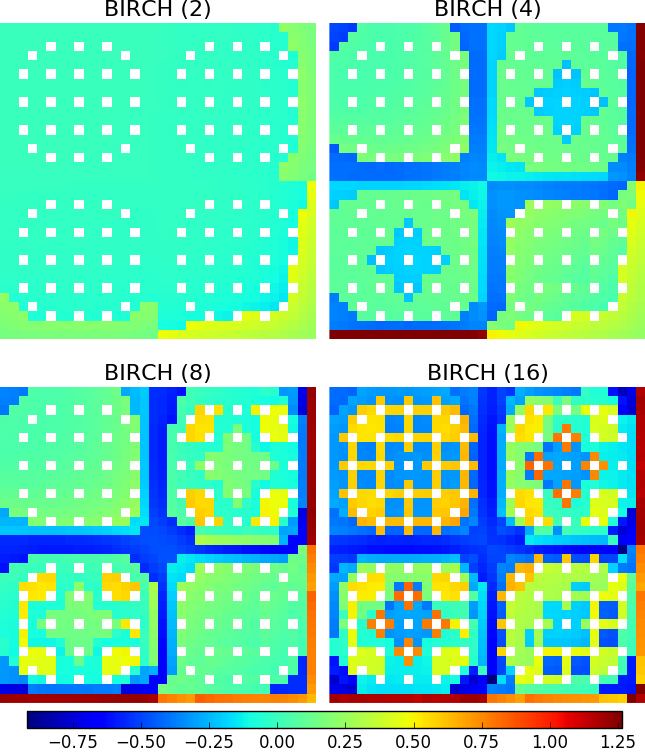
\includegraphics[width=0.63\linewidth]{figures/results/compare/reflector/compare-capt}
\caption[U-238 capture rate comparison for the mini core]{A comparison of U-238 capture rate spatial distributions for \textit{i}MGXS with BIRCH clustering and null spatial homogenization schemes for the 2$\times$2 mini core.}
\label{fig:refl-capt-rates-comp}
\end{figure}

%%%%%%%%%%%%%%%%%%%%%%%%%%%%%%%%%%%%%%%%%%%%%%%%%%%%%%
\subsection*{Pin-Wise Capture-to-Fission Ratios}

As a corollary to the U-238 capture rates, the OpenMOC energy-integrated radiative capture-to-fission ratios were compared to the reference OpenMC capture-to-fission ratios for each homogenization scheme. The spatial distributions of the ratios are plotted as heatmaps for the quarter core BEAVRS model in Fig.~\ref{fig:refl-capt-err} with null and \textit{i}MGXS homogenization with BIRCH clustering of 40 clusters. 

The error is highly structured for the null homogenization scheme since it neglects to account for spatial self-shielding effects of control rod guide tubes and burnable poisons on nearby fuel pins, and from the baffle/reflector on the fuel pins along the core periphery. In contrast, the \textit{i}MGXS scheme ``smooths'' the error distribution for the interior fuel pins. Furthermore, \textit{i}MGXS eliminates the most limiting errors for those fuel pins along the baffle/reflector interface. The residual structural error for the \textit{i}MGXS scheme is gradually removed as more clusters are introduced into the model to account for the varying spatial self-shielding effects throughout the core.

\begin{figure}[h!]
\centering
\begin{subfigure}{0.9\textwidth}
  \centering
  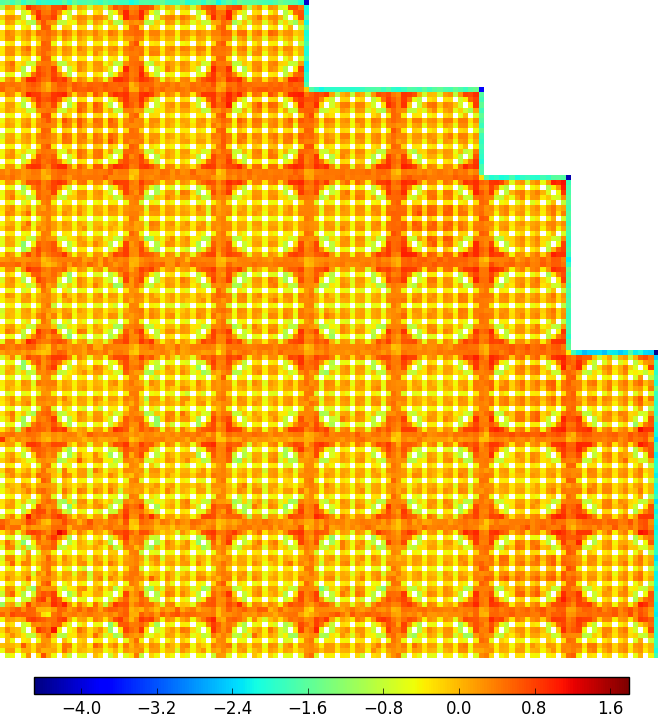
\includegraphics[width=0.65\linewidth]{figures/results/capt-to-fiss/spatial/full-core/capt-to-fiss-err-null}
  \caption{}
  \label{fig:chap11-full-core-capt-err-null}
\end{subfigure}
\begin{subfigure}{0.9\textwidth}
  \centering
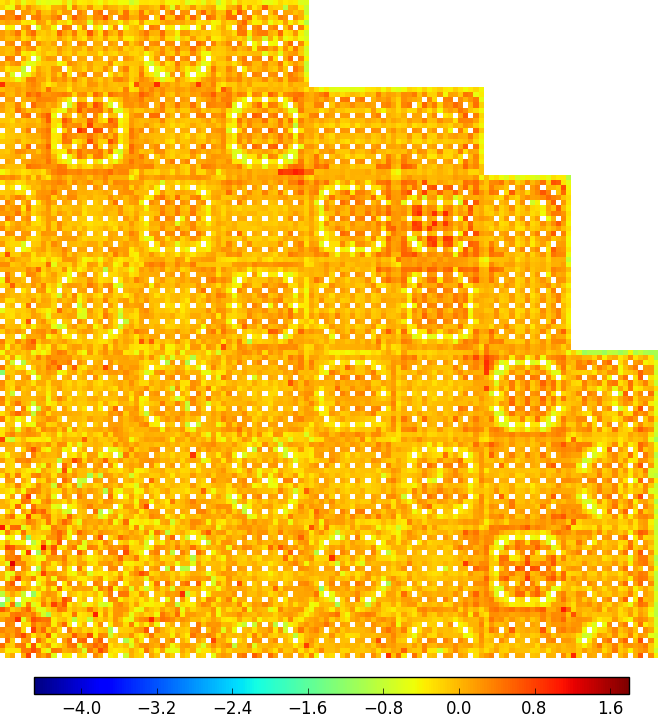
\includegraphics[width=0.65\linewidth]{figures/results/capt-to-fiss/spatial/full-core/capt-to-fiss-err-birch-40}
  \caption{}
  \label{fig:chap11-full-core-capt-err-birch-40}
\end{subfigure}
\caption[Capture-to-fission ratio errors for BEAVRS]{Capture-to-fission percent relative errors for the quarter core BEAVRS model with null homogenization (a) and \textit{i}MGXS homogenization with 20 clusters (b).}
\label{fig:chap11-full-core-capt-err-b}
\end{figure}

%%%%%%%%%%%%%%%%%%%%%%%%%%%%%%%%%%%%%%%%%%%%%%%%
\subsection*{Convergence Rates of MOC Solutions}

This thesis also quantified the number of MC particle histories necessary to sufficiently converge MGXS for stable OpenMOC solutions with each spatial homogenization scheme. OpenMC simulations were used to generate MGXS for varying numbers of particle histories. The MGXS were computed from MC tally data stored as OpenMC \textit{statepoint files} for 100 different active batches (\textit{i.e.}, different numbers of particle histories). The OpenMC statepoints for the earliest batches contained MC tally data with the largest statistical uncertainties, while the tallies for the latter batches had smaller statistical uncertainties. The different statepoints enabled a thorough evaluation of the sensitivity of OpenMOC's solutions to the statistical uncertainties of the MGXS.

The OpenMOC U-238 capture rates were compared to the reference OpenMC capture rates to compute the percent relative errors for each fuel pin for each of the OpenMC statepoints. The relative errors are presented in Fig.~\ref{fig:refl-capture-converge} for the mini core with null, degenerate, LNS and \textit{i}MGXS spatial homogenization with 16 BIRCH clusters. The statistical uncertainty (1-sigma) of the OpenMC estimate for the pin-wise U-238 capture rates is also highlighted in each figure to quantify how much faster a solution for a specified accuracy can be achieved with OpenMOC with MGXS generated by OpenMC.

The OpenMC uncertainties approach zero while the OpenMOC errors approach a non-zero bias dependent on the approximation error related to OpenMOC's numerical discretization. The convergence of the \textit{i}MGXS scheme lies between that of the null and degenerate schemes, and requires more particle histories to converge as more clusters are identified. The converged \textit{i}MGXS errors increasingly approach the degenerate errors as more clusters are introduced. \textbf{The figures illustrate that \textit{i}MGXS achieves nearly the same accuracy as the degenerate scheme with a factor of at least ten fewer particle histories. Furthermore, the results indicate that OpenMOC's errors converge at least an order of magnitude faster than OpenMC's statistical uncertainties.}
 
\begin{figure}[h!]
\centering
\begin{subfigure}{\textwidth}
  \centering
  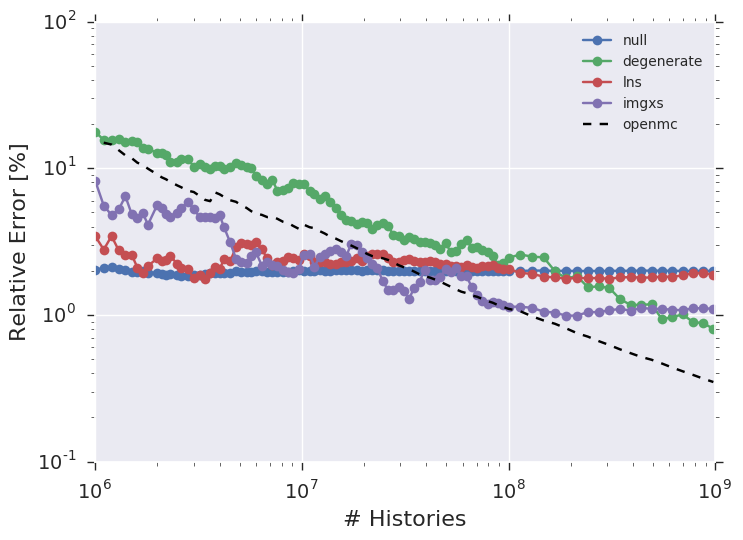
\includegraphics[width=0.9\linewidth]{figures/results/convergence/reflector/max-capt-err-evo-exec-summary}
  \caption{}
  \label{fig:refl-max-converge}
\end{subfigure}
\begin{subfigure}{\textwidth}
  \centering
  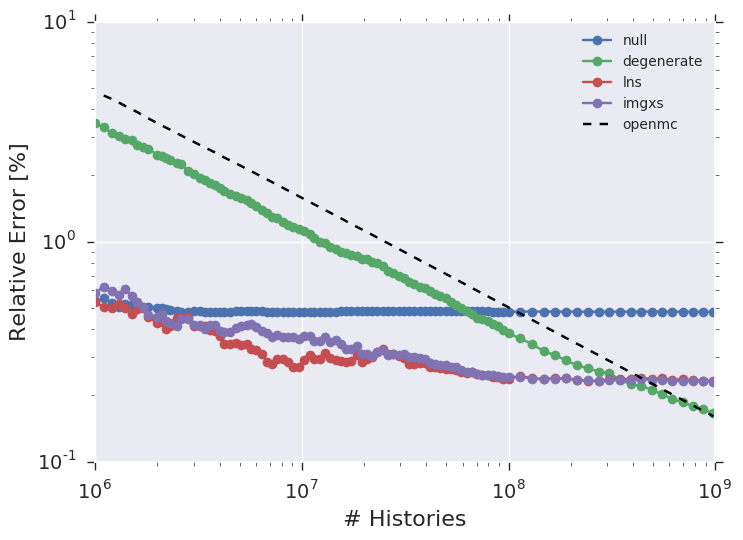
\includegraphics[width=0.9\linewidth]{figures/results/convergence/reflector/mean-capt-err-evo-exec-summary}
  \caption{}
  \label{fig:refl-mean-converge}
\end{subfigure}
\vspace{2mm}
\caption[Fission rate covergence for the 2$\times$2 mini core]{Convergence of the max (a) and mean (b) absolute U-238 capture rate percent relative errors for the 2$\times$2 mini core.}
\label{fig:refl-capture-converge}
\end{figure}

\clearpage

%%%%%%%%%%%%%%%%%%%%%%%%%%%%%%%%%%%%%%%%%%%%%%%%%%%%%%%%%%%%%%%%%%%%%%%%%%%%%%%%
\section*{Conclusions}

This thesis had two primary goals: to quantify approximation error in MGXS and to develop new spatial homogenization methods to accelerate the convergence of MGXS on heterogeneous MC tally meshes. These goals were motivated by the desire to obtain Monte Carlo-quality solutions with computationally efficient deterministic neutron transport methods. The following summarizes the key accomplishments demonstrated by this thesis to meet this over-arching vision:

%This was accomplished with a simulation framework that evaluated the MGXS generated by stochastic transport simulations with OpenMC for use in deterministic multi-group transport simulations with OpenMOC. The \textit{i}MGXS spatial homogenization scheme was developed to directly model all energy and spatial self-shielding effects to generate accurate MGXS with a single whole-core MC calculation. 

%This thesis had two primary goals: to quantify approximation error in MGXS and to develop new spatial homogenization methods to accelerate the convergence of MGXS on heterogeneous MC tally meshes. This was accomplished with a simulation framework that evaluated the MGXS generated by stochastic transport simulations with OpenMC for use in deterministic multi-group transport simulations with OpenMOC. The \textit{i}MGXS spatial homogenization scheme was developed to directly model all energy and spatial self-shielding effects to generate accurate MGXS with a single whole-core MC calculation. 

\begin{itemize}

\item \textbf{Design and implementation of software simulation infrastructure.} The simulation framework replaces the multi-level approach to directly model all energy and spatial self-shielding with a single whole-core OpenMC calculation of the complete heterogeneous geometry to generate MGXS for use in OpenMOC.

\item \textbf{Systematic evaluation of bias between OpenMC and OpenMOC.} The approximations made to collapse MGXS in energy, space and angle were quantified for simple PWR benchmarks. The impact of the flux separability approximation was rigorously quantified, and a method based on SuPerHomog\'{e}n\'{e}isation factors was implemented to ensure reaction rate consistency between OpenMC and OpenMOC.

\item \textbf{Design and implementation of pin-wise spatial homogenization schemes.} The LNS scheme uses an engineering-based nearest of a reactor's geometric configuration to assign MGXS to each fuel pin. The \textit{i}MGXS scheme uses machine learning to detect MGXS clustering in ``noisy'' MC tally data, and assigns MGXS to fuel pins without any knowledge of a reactor's geometric configuration.

%\item \textbf{Design and implementation of pin-wise spatial homogenization schemes.} The LNS scheme employs an engineering-based nearest neighbor analysis of the geometric configuration of a reactor core to assign MGXS to each fuel pin. The iMGXS scheme uses unsupervised machine learning methods to detect MGXS clustering in ``noisy'' MC tally data and infer the optimal assignment of MGXS to each fuel pin.



\item \textbf{Quantified the predictive accuracy of the LNS and \textit{i}MGXS schemes.} Both schemes were shown to reduce pin-wise U-238 capture rate errors by a factor of four by adequately accounting for spatial self-shielding effects from core heterogeneities. The \textit{i}MGXS scheme performed better than LNS for fuel pins along assembly-assembly and assembly-reflector interfaces. 

%The iMGXS scheme achieves the same accuracy as LNS with up to two orders of magnitude fewer MGXS clusters for the quarter core BEAVRS model.

%The OpenMOC solutions were compared to reference solutions generated with OpenMC for six heterogeneous PWR benchmarks. Both schemes reduced errors for U-238 capture rates predicted by OpenMOC relative to a reference OpenMC solution by a factor four. The iMGXS scheme 

\item \textbf{Quantified the MC histories needed to converge the MGXS for each scheme.} Both schemes were shown to require at least an order of magnitude fewer MC particle histories to converge MGXS for accurate deterministic calculations than a reference MC calculation. 

%\item Designed and implemented software framework to generate MGXS with OpenMC for use in OpenMOC. The simulation framework replaces the multi-level approach to model self-shielding with a single whole-core OpenMC calculation of the complete heterogeneous geometry to generate MGXS for use in OpenMOC.

%\item Designed inferential multi-group cross section methodology for pin-wise spatial homogenization of MGXS. The iMGXS data processing pipeline uses machine learning methods to detect MGXS clustering in ``noisy'' MC tally data and infer the optimal assignment of fuel pins to spatial homogenization zones.
\end{itemize}

%These goals were motivated by the desire to obtain Monte Carlo-quality solutions with computationally efficient deterministic neutron transport methods.

%The \textit{i}MGXS scheme is a data processing pipeline which uses machine learning algorithms to infer the clustering of MGXS in fuel pins due to spatial self-shielding effects with limited supervision or engineering domain knowledge.

%The \textit{i}MGXS scheme was demonstrated to identify spatial self-shielding effects from ``noisy'' MC tally data without any knowledge of a reactor's geometric configuration. The scheme was shown to reduce pin-wise U-238 capture rate errors by a factor of four by adequately accounting for spatial self-shielding effects from core heterogeneities including control rod guide tubes, burnable poisons, and reflectors with on the order of only ten MGXS clusters. Furthermore, the \textit{i}MGXS scheme was shown to be advantageous over geometric heuristic approaches such as LNS which must be highly customized for specific types of core geometries, and which fail to distinguish MGXS clusters for pins at assembly-assembly and assembly-reflector interfaces. Finally, the \textit{i}MGXS scheme was shown to require at least an order of magnitude fewer MC particle histories to converge MGXS for accurate deterministic calculations than a reference MC calculation. 

%\textbf{The \textit{i}MGXS scheme enables deterministic reactor physics simulations to produce accurate results from MGXS generated by MC faster than would be possible with a direct calculation with MC.} This thesis demonstrated the promise for \textit{i}MGXS as a means to efficiently generate MGXS with reactor agnostic MC calculations of the complete heterogeneous geometry in a single step.

\textbf{The \textit{i}MGXS scheme enables deterministic reactor physics simulations to produce accurate results from MGXS generated by MC faster than would be possible with a direct calculation with MC.} Furthermore, the \textit{i}MGXS scheme was shown to be advantageous over geometric heuristic approaches such as LNS which must be highly customized for specific types of core geometries. This thesis demonstrated the promise for \textit{i}MGXS as a means to efficiently generate MGXS with reactor agnostic MC calculations of the complete heterogeneous geometry in a single step.

%%%%%%%%%%%%%%%%%%%%%%%%%%%%%%%%%%%%%%%%%%%%%%%%%%%%%%%%%%%%%%%%%%%%%%%%%%%%%%%%
\section*{Future Work}

This thesis identified several issues which must be investigated in the future in order for \textit{i}MGXS to be useful in a production code setting. First, a systematic evaluation of the types of features, as well as algorithms for dimensionality reduction and clustering, which may be used in \textit{i}MGXS should be performed to better understand their impact on the resulting clustered geometry. A future study should also score each configuration of the \textit{i}MGXS data processing pipeline based on how many MC particle histories  each scheme requires to accurately identify MGXS clusters from ``noisy'' MC tally data. 

Future work should also consider employing \textit{i}MGXS in calculations with thermal-hydraulic feedback and nuclide depletion where the moderator density, fuel temperature and burnup will be needed as features to predict MGXS clustering. In addition, new methods must be developed to compute transport-corrected MGXS with MC which appropriately account for anisotropic scattering, thereby eliminating the isotropic in lab scattering approximations used throughout this work. Finally, this thesis may serve as inspiration to employ machine learning algorithms to automate the time-consuming process of selecting reduced energy group structures and their optimal energy group boundaries for MGXS.

%evaluate \textit{i}MGXS scheme:
%-add anisotropic scattering to OpenMOC to enable solution of the ``correct'' problem
%-systematic study of featues -- ones actually matter? \\
%-systematic study to understand impact of dimensionality reduction \\
%-systematic study to understand impact of clustering algorithms \\
%-more research into model selection schemes -- none of them robustly works for my case studies! \\
%-evaluate \textit{i}MGXS with clustering ``on-the-fly'' with noisy MC tally data \\
%-can \textit{i}MGXS reduce the number of necessary energy groups?? \\

%reach goals:\\
%-multi-physics applications: moderator density, fuel temperature, burnup, etc. as features \\
%-machine learning to optimize energy group structures \\

%-speed up OpenMOC full core: \\
%  -find a way use quarter assembly CMFD mesh \\
%  -linear source to reduce number of spatial zones \\
%  -vectorize transport solver over energy groups \\


%%%%%%%%%%%%%%%%%%%%%%%%%%%%%%%%%%%%%%%%%%%%%%%%%%%%%%%%%%%%%%%%%%%%%%%%%%%%%%%%
%%%%%%%%%%%%%%%%%%%%%%%%%%%%%%%%%%%%%%%%%%%%%%%%%%%%%%%%%%%%%%%%%%%%%%%%%%%%%%%%
% BIBLIOGRAPHY

\begin{singlespace}
\bibliographystyle{ans}
\bibliography{references}
\end{singlespace}

\end{document}
